\documentclass[12pt,a4paper]{report}
\usepackage[top=0.70in, bottom=0.70in, left=0.8in,right=0.80in]{geometry} % 
\usepackage[pdftex]{graphicx} %for embedding images
\usepackage[%dvips, % commented for pdflatex
bookmarks,  colorlinks=false]{hyperref}
\hypersetup{%
    pdfborder = {0 0 0}
}
\usepackage{verbatim}
\usepackage[final]{pdfpages} 
\usepackage{float}
\usepackage{hyperref}
\usepackage{pslatex}
\usepackage{array}
\usepackage{setspace}
\usepackage{float}
\usepackage{enumerate}
\usepackage{longtable}
\usepackage[font=small,labelfont=bf]{caption}
\def\figurename{\textbf{Figure }}
\usepackage{fancyhdr}
\fancypagestyle{plain}{%
\fancyfoot[L]{\emph{Ingeniería de Software}} % except the center
\fancyfoot[R]{\thepage}
\renewcommand{\headrulewidth}{0.4pt}
\renewcommand{\footrulewidth}{0.4pt}
}
\pagestyle{fancy}
\rhead{\emph{Sistema de Administraci\'on Escolar}}
\fancyfoot[LO,LE]{\emph{Ingenier\'ia de Software}}
\cfoot{}
\fancyfoot[RO, RE]{\thepage}
\renewcommand{\headrulewidth}{0.4pt}
\renewcommand{\footrulewidth}{0.4pt}
\usepackage{pgf}
\usepackage{pgfpages}
\pgfpagesdeclarelayout{boxed}
{
  \edef\pgfpageoptionborder{0pt}
}
{
  \pgfpagesphysicalpageoptions
  {%
    logical pages=0,%
  }
  \pgfpageslogicalpageoptions{1}
  {
    border code=\pgfsetlinewidth{2pt}\pgfstroke,%
    border shrink=\pgfpageoptionborder,%
    resized width=.95\pgfphysicalwidth,%
    resized height=.95\pgfphysicalheight,%
    center=\pgfpoint{.5\pgfphysicalwidth}{.5\pgfphysicalheight}%
  }%
}
\pgfpagesuselayout{boxed}
\setlength{\parindent}{1cm}
\usepackage[utf8]{inputenc}
\usepackage[spanish]{babel} 

\begin{document}
\renewcommand\bibname{References}
\lhead{ }

\newpage
\begin{center}
\thispagestyle{empty}
\LARGE{\textsc {\textbf{INSTITUTO POLITÉCNICO NACIONAL}}}\\[0.5cm]
\Large{\textbf{ESCUELA SUPERIOR DE CÓMPUTO}}\\[0.7cm]
\vspace{5cm}
\Large{\textbf{\\PROYECTO}}
\LARGE{\textbf{\\Sistema de Administración Escolar: SAES\\}}
\vspace{7cm}
\end{center}
\Large{\textbf{\\INGENIERÍA DE SOFTWARE}}
\vspace{5cm}
\begin{flushright}
\Large{\textbf{\\17 de Septiembre de 2017}}
\end{flushright}
\newpage
\newpage
\newpage
\begin{center}
\thispagestyle{empty}
\LARGE{\textsc {\textbf{INSTITUTO POLITÉCNICO NACIONAL}}}\\[0.5cm]
\Large{\textbf{ESCUELA SUPERIOR DE CÓMPUTO}}\\[0.7cm]
\vspace{0.5cm}
\Large{\textbf{\\PROYECTO}}
\LARGE{\textbf{\\``Sistema de Administración Escolar: SAES''\\}}
\vspace{2cm}
\Large{\textbf{\\INGENIERÍA DE SOFTWARE}}
\vspace{2cm}
\end{center}
\Large{\textbf{\\INTEGRANTES}}\\
\large{
\begin{itemize}
    \item BELTRÁN ALVARADO ROGELIO
    \item ESTRADA GRANADOS DIEGO
    \item HERNÁNDEZ PINEDA MIGUEL ANGEL
    \item HUITRÓN RIZO GABRIEL ALEJANDRO
    \item MATUS LÓPEZ CARLOS EDUARDO
    \item MEDINA LUQUEÑO ANA XIMENA
    \item MONROY MARTOS ELIOTH
    \item MONSALVO FUENTES AMÉRICA BERENICE
    \item OSORNIO DÍAZ EMILIANO
    \item PAREDES RIVAS ALBERTO
    \item TREJO GRANADOS YAHIR
\end{itemize}
}
\vspace*{1cm}
\large{\textbf{PROF. IDALIA CASTILLO MALDONADO}}\\
\newpage
\newpage
\begin{center}
\thispagestyle{empty}
\vspace{2cm}
\LARGE{\textbf{OBJETIVO}}\\[1.0cm]
\end{center}
\thispagestyle{empty}
\large{\paragraph{}Realizar una mejora al Sistema de Administración Escolar (SAES) del Instituto Politécnico Nacional en el módulo de reinscripción para poder llevar a cabo el proceso de reinscripción de los alumnos de una manera mas fácil y rápida.}
\newpage

\pagenumbering{roman}
\pagestyle{empty}
\addtocontents{toc}{\protect\thispagestyle{empty}}
\tableofcontents
\addtocontents{lof}{\protect\thispagestyle{empty}}
\listoffigures
\cleardoublepage

\pagestyle{fancy}
\newpage
\pagenumbering{arabic}

%\input{project/introduction.tex}
\chapter{Ámbito del Software}
\noindent
El módulo de reinscripción del Sistema de Administración Escolar (en adelante SAES) del Instituto Politécnico Nacional (en adelante IPN) se volverá a hacer añadiendo mejoras y corrigiendo los errores que se presentan en el mismo actualmente.\\
El proyecto se desarrollará desde la fase de análisis hasta la fase de pruebas, por lo que será necesario tener algunos otros módulos como el registro de los distintos tipos de usuario, así como algunas funciones de estos; tendremos los módulos de registro de alumno y administrador, así como el de iniciar sesión, además es necesario contar con algunas de las funciones del administrador para poder llevar a cabo el registro de materias, profesores y otros datos.
Centrándonos en el módulo de reinscripción, se trabajará en el basándonos estrictamente según las normas establecidas en el Reglamento General de Estudios del IPN donde se definen algunos criterios a considerar para poder llevar a cabo este proceso.\\
Las funciones esenciales del alumno serán todas las relacionadas con la reinscripción tomando algunas de las que ya han sido establecidas en el módulo actual, así como nuevas funciones que permitan una mejor navegación y manejo de las distintas secciones dentro del sistema.\\
El sistema le permitirá al alumno buscar información de las materias del semestre al que se va a inscribir un par de semanas antes de que llegue la fecha de inscripciones, en ese mismo momento será posible llevar a cabo el armado de uno o varios horarios tentativos de acuerdo a sus preferencias para que llegada su cita de inscripción verifique si puede inscribir alguno de estos, además, para hacer más ágil este proceso se contarán con diferentes filtros para que la búsqueda de materias, profesores o grupos sea más fácil durante este proceso; se llevarán a cabo las validaciones pertinentes para informarle al alumno si es posible reinscribirse a través del SAES, en caso de que no se le permita, el sistema le informará que debe acudir a la oficina de gestión escolar de su unidad académica para llevar a cabo este proceso. 
\newpage
\noindent
De acuerdo a lo establecido actualmente, las citas de reinscripción se generarán según el promedio del alumno, teniendo prioridad los alumnos con un mejor promedio. Durante el proceso de reinscripción, el alumno será capaz de administrar las materias que desea inscribir, es decir, podrá agregar o eliminar materias a su lista de reinscripción, de acuerdo a los créditos que tenga disponibles, antes de que verifique y termine con su reinscripción.\\
Finalmente, el sistema le mostrará, durante el periodo de reinscripción, diferentes opciones de horario al alumno de acuerdo al semestre que cursará y basándose en la información de los cupos de cada materia en el momento, así como en el horario asignado a cada una de estas, reduciendo así, las horas muertas se verán reducidas en estas opciones, es importante resaltar que solo son recomendaciones o sugerencias para el alumno por lo que es su decisión si desea inscribir o no el horario. 

\chapter{Análisis de Requerimientos}
\section{Requisitos Funcionales}
\begin{enumerate}[{RF} 1.]
\item El sistema contará con perfiles de alumno y administrativo.
\item El sistema permitirá el acceso mediante el id del usuario y la contraseña correspondiente.
\item El sistema permitirá al alumno restablecer su contraseña mediante el envío de un enlace temporal a una dirección web que le permita asignar una nueva contraseña. 
\item El sistema permitirá al usuario de tipo administrador gestionar la información de: alumnos, materias (Plan de estudios 09), grupos y profesores.
\item El sistema mostrará al alumno su historial académico.
\item El sistema determinará el estado del alumno con base en su historial académico.
\item El sistema informará al alumno si puede llevar a cabo o no su reinscripción en linea, cuando se le asigne una cita de reinscripción.
\item El administrador podrá habilitar o deshabilitar el proceso de reinscripción con base en el calendario escolarizado del IPN.
\item El sistema permitirá la inscripción y reinscripción de alumnos.
\item El sistema será capaz de realizar búsquedas de materias disponibles para la reinscripción con base en el nombre de la materia, nombre del profesor, grupo y nivel de la materia.
\item El sistema permitirá observar al alumno la disponibilidad de materias durante el periodo de reinscripción con base en el nombre de la materia, nombre del profesor, grupo y nivel.
\item El sistema permitirá al alumno elegir entre una serie de horarios generados a partir del turno en el que desea inscribirse así como en la disponibilidad de los grupos al momento de su inscripción.
\item El sistema le permitirá al usuario crear diferentes horarios desde 2 semanas antes de la fecha de reinscripción.
\item El sistema permitirá al usuario inscribir un horario previamente diseñado como horario de clases a la hora de su inscripción.
\item El sistema permitirá al usuario seleccionar una materia para ser inscrita durante su proceso de inscripción.
\item El sistema permitirá al usuario eliminar una materia inscrita previamente a su horario de clases antes de finalizar su reinscripción.
\item El sistema no permitirá inscribir al alumno una materia con el mismo horario que alguna otra seleccionada anteriormente.
\item El sistema no permitirá al alumno inscribir materias que se encuentren seriadas con alguna materia que no ha sido cursada por el alumno.
\item El sistema permitirá al alumno inscribir una materia seriada solo si la materia que serializa a esta ha sido aprobada.
\item El sistema permitirá al alumno finalizar su reinscripción y visualizar su horario inscrito.
\end{enumerate}
\newpage
\section{Requisitos No Funcionales}
\begin{enumerate}[{RNF} 1.]
\item Usabilidad, el sistema contará con un diseño amigable e intuitivo otorgando al usuario un fácil uso y una grata experiencia.
\item Usabilidad, el sistema proporcionará los mensajes adecuados a cada caso que se enfrente el usuario.
\item Estabilidad, el sistema funcionará de manera correcta siempre que el usuario haga uso de él.
\item Operatividad, el sistema cumplirá con el objetivo y los requisitos planteados.
\item Mantenibilidad, si el sistema requiere de alguna mejora futura, debido a la organización.
\item Disponibilidad, el sistema será accesible en todo momento para los distintos usuarios del mismo.
\item Accesibilidad, el sistema será accesible desde cualquier navegador moderno, permitiendo así a los usuarios acceder desde cualquier dispositivo inteligente.
\item Concurrencia, el sistema permitirá a más de un usuario acceder al mismo tiempo.
\end{enumerate}
\newpage
\section{Reglas de Negocio}
\begin{enumerate}[{RN} 1.]
\item El alumno tiene que contar con un número de boleta proporcionado por el Instituto Politécnico Nacional para poder entrar al sistema
\item La contraseña establecida por el alumno debe tener más de 6 caracteres, una letra mayúscula, una letra minúscula, un número y un caracter especial.
\item Para la reinscripción, el alumno deberá considerar el resultado de dividir el total de los créditos faltantes para concluir su plan de estudio, entre los periodos escolares disponibles para completarlo. Si el resultado de la división es menor o igual a la carga media definida en el plan de estudio, el alumno tendrá derecho a reinscripción conforme a las reglas siguientes:
\item El alumno tendrá que inscribirse en el rango de créditos presentados por el mapa curricular de la institución.
\item Cuando el alumno solicite reinscribirse a una carga menor a la mínima o mayor a la máxima, deberá presentar por escrito una solicitud justificada  al titular de la unidad académica para obtener la autorización correspondiente.
\item Si el alumno adeuda más de 3 materias, no podrá reinscribirse a través del sistema, tendrá que llevar a cabo dicho proceso en la oficina de Gestión Escolar. 
\item El alumno que cuente con adeudos de unidades de aprendizaje tendrá derecho a recursarlas solo una vez.
\item En caso de presentarse recurses, el alumno no podrá rebasar la carga media de créditos.
\item Si el alumno adeuda una unidad de aprendizaje de cualquier otro periodo escolar y solicita reinscribirse a una carga menor a la mínima, deberá presentar por escrito una solicitud justificada a la Comisión de Situación Escolar del Consejo Técnico Consultivo Escolar.
\item Si el resultado de la división referida en la regla de negocio 2, es mayor a la carga media definida en el plan de estudio, esto implica que no podrá concluir sus estudios en el plazo máximo establecido en el plan de estudio, por lo que deberá solicitar ante la Comisión de Situación Escolar del Consejo General Consultivo la autorización de reinscripción y, en su caso, ampliación de plazo para la conclusión del plan de estudio.
\item Un profesor no puede tener más de 1 materia en el mismo horario.
\item Un profesor sólo puede ser asignado a materias del área del conocimiento correspondiente a los conocimientos del mismo.
\item Una materia no puede asignarse al mismo grupo más de una vez.
\item En un mismo grupo no puede haber 2 o mas materias con el mismo horario.
\item Los créditos de una unidad de aprendizaje van de 1.5 a 13.0
\item El Alumno no podrá inscribir en un mismo periodo dos o más materias con el mismo nombre.
\item El Alumno no podrá inscribir en un mismo periodo dos o más materias con el mismo horario. 
\item El periodo de reinscripciones deberá de ser de al menos 3 días de duración.
\end{enumerate}
\section{Mensajes}
\subsection{Mensajes de Alerta}
\begin{enumerate}[{MA} 1.]
\item ¿Estás seguro al dar de baja la materia seleccionada?
\item ¿Estás seguro que quieres finalizar tu inscripción?
\item No cuentas con materias inscritas en este momento
\item ¿Deseas inscribir otra materia?
\item No tienes grupos-materias asignados en este semestre.
\item No hay alumnos inscritos <<grupo seleccionado>> - <<materia seleccionada>> aún.
\end{enumerate}
\subsection{Mensajes de Confirmación}
\begin{enumerate} [{MC} 1.]
\item El <<registro actual>> se registró correctamente.
\item Se ha enviado un correo para la restauración de la contraseña al correo asociado con la cuenta.
\item Se actualizaron los datos correctamente.
\item Se generaron todas las citas de inscripción correctamente.
\item Se concluyó la inscripción correctamente.
\item Se registró la solicitud de dictamen de manera correcta.
\item Se agregó correctamente el tipo de horario
\end{enumerate}
\newpage
\subsection{Mensajes de Error}
\begin{enumerate}[{ME} 1.]
\item Se dejaron campos obligatorios en blanco
\item El correo está registrado en otra cuenta
\item Lo sentimos, el número de boleta ya fue asignado a otro alumno
\item El número de empleado ya fue asignado a otra cuenta
\item No hay cuenta asociada a este usuario. Ingrese un usuario válido
\item No hay materias registradas
\item No hay profesores del área registrados
\item No hay grupos registrados
\item No hay horarios registrados
\item No se aceptan duplicados de materias en un mismo grupo
\item No se aceptan duplicados de horarios para un mismo profesor
\item El horario no está disponible, seleccione otro
\item No se generaron todas la citas de reinscripción correctamente
\item El número de boleta no existe.
\item Lo sentimos, ya no hay cupo
\item Se genera un traslape de materias, por favor escoge la materia en otro horario
\item Ya has agregado una materia con el mismo nombre
\item Ya no cuenta con mas periodos escolares para concluir su carrera. Favor de checar su situación académica
\item La materia ya ha sido cursada y aprobada, no es posible inscribirla.
\item La cita de reinscripción expiró
\item No se han seleccionado materias
\item El grupo ya ha sido registrado, por favor ingrese otro valor.
\item La búsqueda no obtuvo resultados.
\item La materia ya ha sido recursada, no puedes inscribirla de nuevo.
\item No se encuentra en el rango de créditos.
\item La fecha de fin del periodo de reinscripciones debe ser posterior a la fecha de inicio.
\item La hora de fin por día del periodo de reinscripciones debe ser posterior a la hora de inicio.
\item El periodo de reinscripciones debe ser de al menos 3 días.
\item No se encontraron resultados.
\item El grupo ingresado no existe.
\item Extiende este texto para que tenga 6 caracteres o más (actualmente usas <<número de caracteres ingresados>> carácter).
\item El usuario o la contraseña son incorrectos.
\item Haz coincidir el formato solicitado.
\item Ya se tiene registrado un horario con este nombre
\item Completa este campo
\item Utiliza un formato que coincida con el solicitado <<formato solicitado>>
\item Incluye un signo ''@''  en la dirección de correo electrónico. La dirección <<dirección actual>> no incluye el signo ''@''
\item Introduce texto detrás del signo ''@''. La dirección <<dirección actual>> esta incompleta.
\item El RFC ya existe.
\item Contraseña incorrecta
\item Las contraseñas no coinciden
\end{enumerate} 
\chapter{Diseño de las Interfaces}
\begin{figure}[H]
  \centering
    \includegraphics[scale=0.2]{project/images/1.png}
  \caption{\textbf{Inicio}}
\end{figure}
\begin{figure}[H]
  \centering
    \includegraphics[scale=0.2]{project/images/2.png}
  \caption{\textbf{Login}}
\end{figure}
\begin{figure}[H]
  \centering
    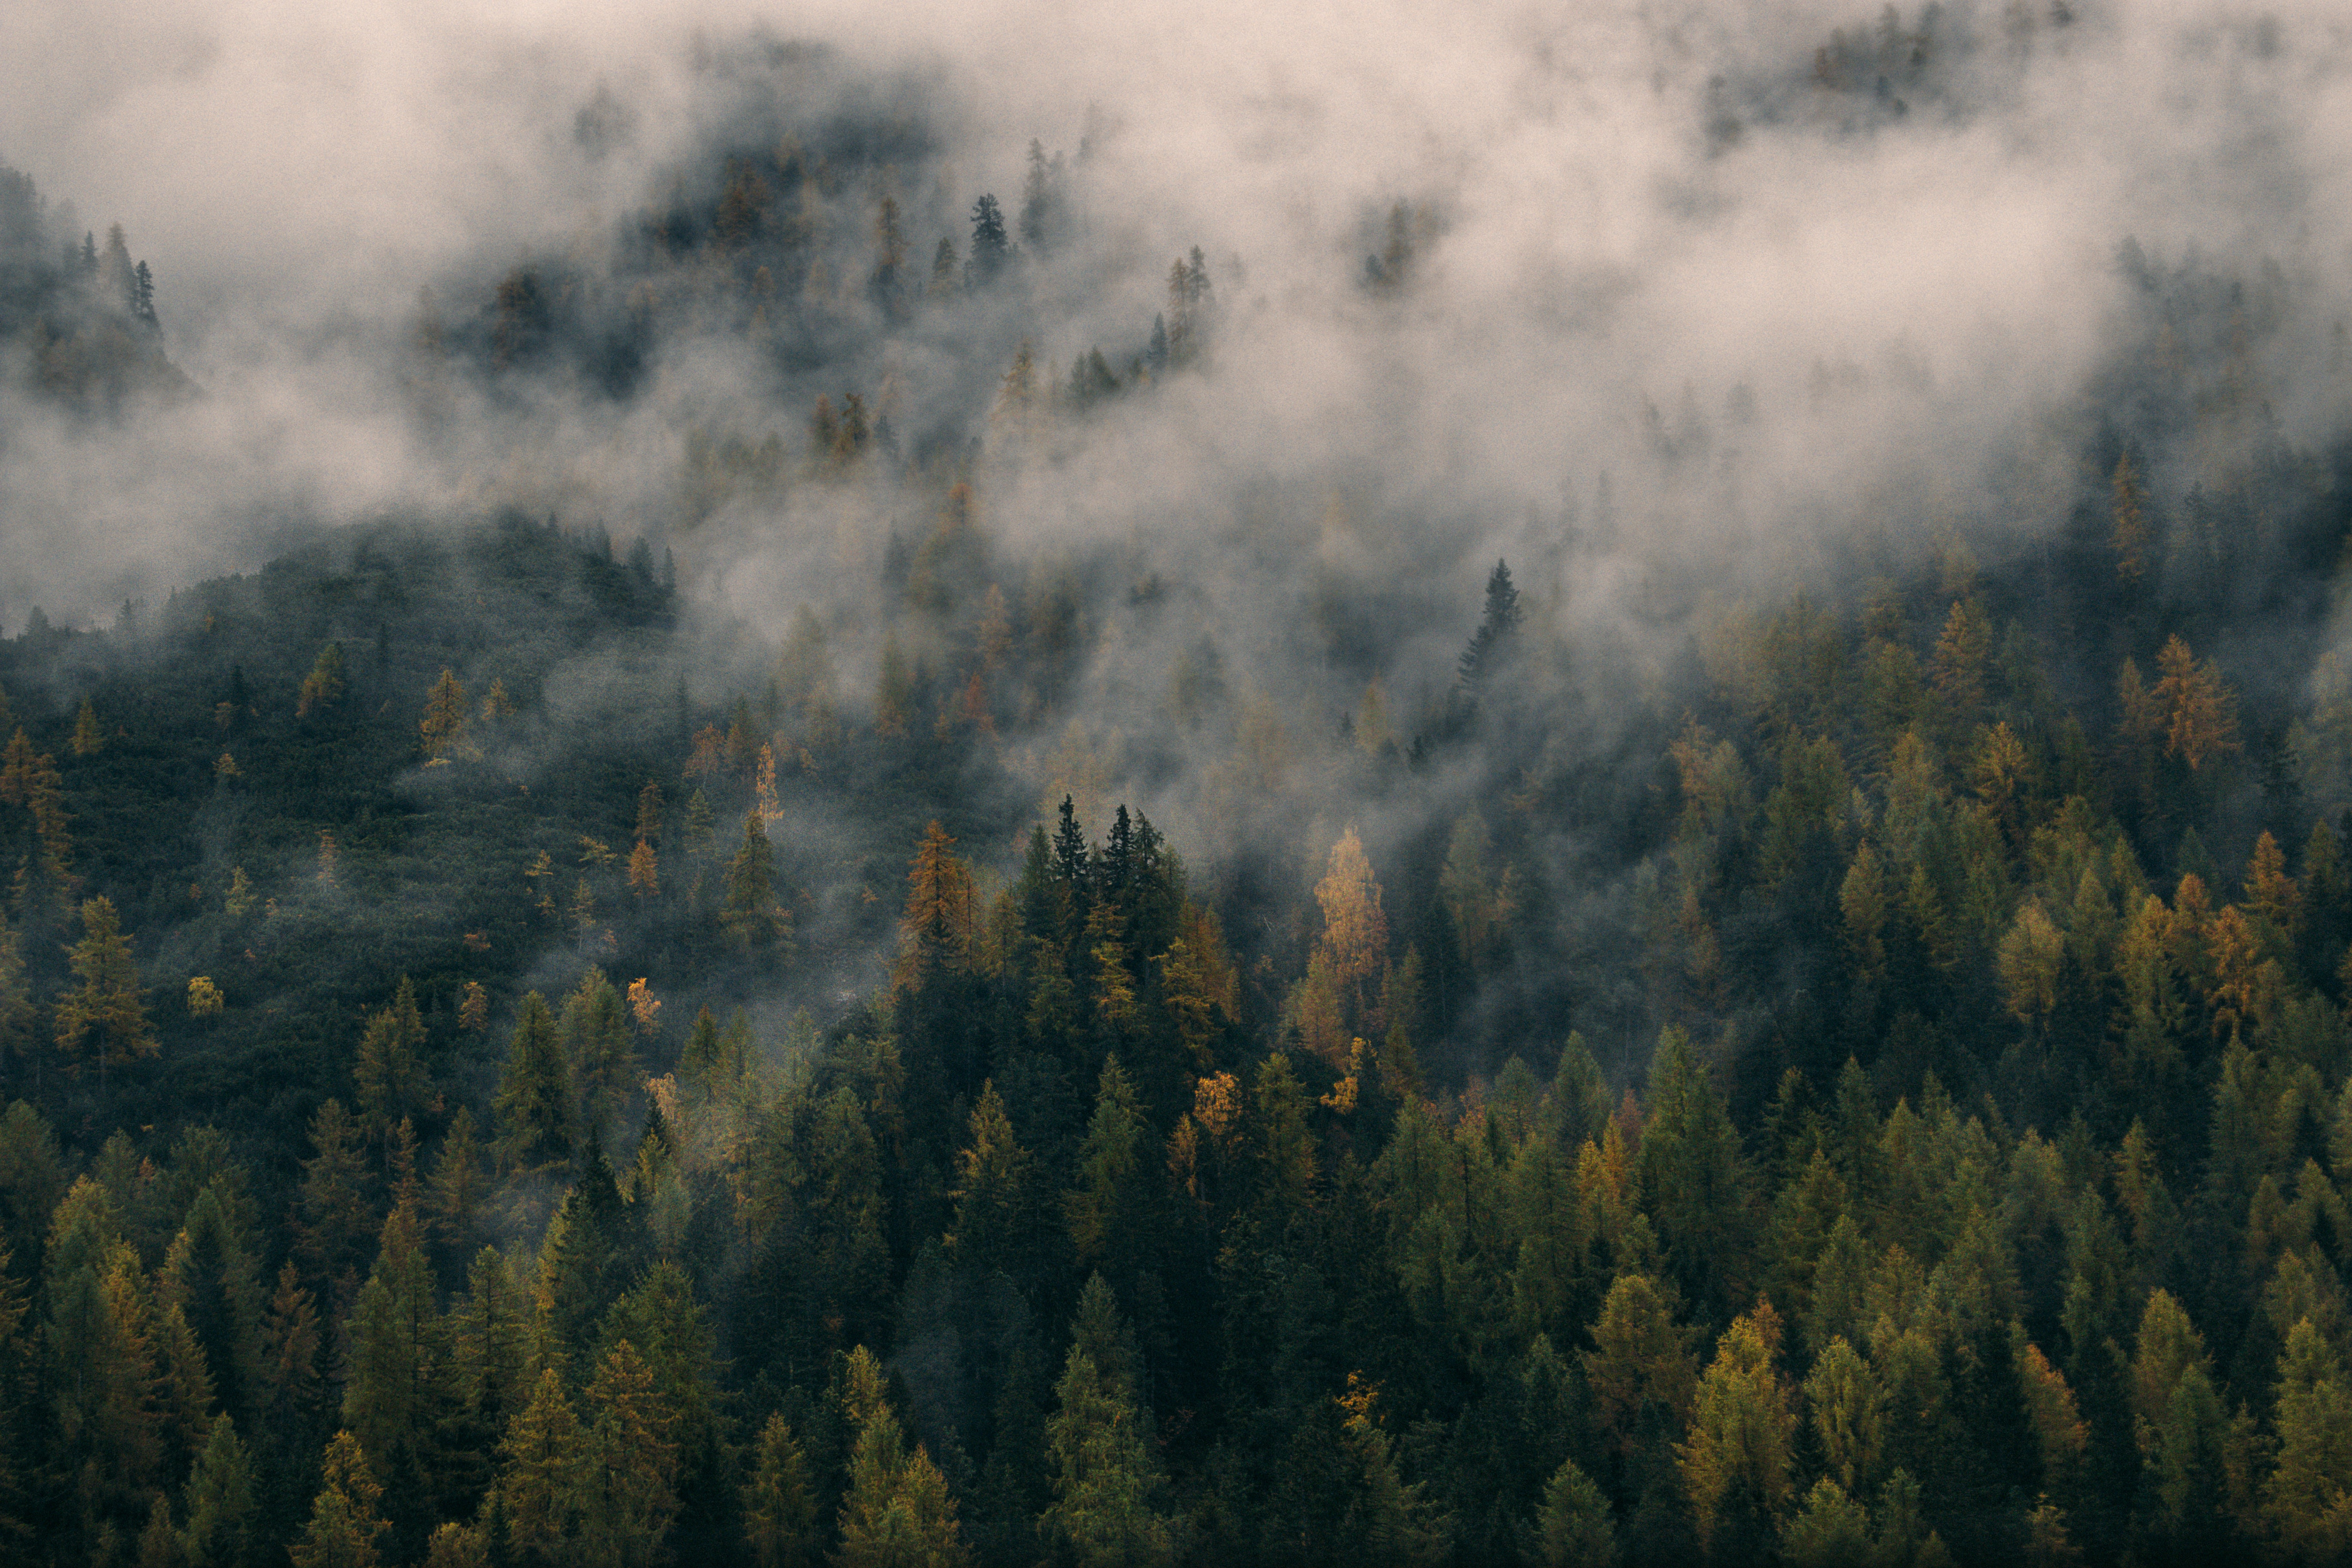
\includegraphics[scale=0.2]{project/images/15.png}
  \caption{\textbf{Datos Generales: Jefe de Gestión Escolar}}
\end{figure}
\begin{figure}[H]
  \centering
    \includegraphics[scale=0.2]{project/images/19.png}
  \caption{\textbf{Registrar Alumno: Jefe de Gestión Escolar}}
\end{figure}
\begin{figure}[H]
  \centering
    \includegraphics[scale=0.2]{project/images/17.png}
  \caption{\textbf{Registrar Analista}}
\end{figure}
\begin{figure}[H]
  \centering
    \includegraphics[scale=0.2]{project/images/16.png}
  \caption{\textbf{Registrar Académico: Jefe de Gestión Escolar}}
\end{figure}
\begin{figure}[H]
  \centering
    \includegraphics[scale=0.2]{project/images/18.png}
  \caption{\textbf{Registrar Profesor: Jefe de Gestión Escolar}}
\end{figure}
\begin{figure}[H]
  \centering
    \includegraphics[scale=0.2]{project/images/20.png}
  \caption{\textbf{Asignar Horario: Jefe de Gestión Escolar}}
\end{figure}
\begin{figure}[H]
  \centering
    \includegraphics[scale=0.2]{project/images/27.png}
  \caption{\textbf{Administrar Alumno: Jefe de Gestión Escolar}}
\end{figure}
\begin{figure}[H]
  \centering
    \includegraphics[scale=0.15]{project/images/55.png}
  \caption{\textbf{Editar Alumno: Jefe de Gestión Escolar}}
\end{figure}
\begin{figure}[H]
  \centering
    \includegraphics[scale=0.2]{project/images/23.png}
  \caption{\textbf{Administrar Analista}}
\end{figure}
\begin{figure}[H]
  \centering
    \includegraphics[scale=0.2]{project/images/24.png}
  \caption{\textbf{Editar Analista}}
\end{figure}
\begin{figure}[H]
  \centering
    \includegraphics[scale=0.2]{project/images/21.png}
  \caption{\textbf{Administrar Académico: Jefe de Gestión Escolar}}
\end{figure}
\begin{figure}[H]
  \centering
    \includegraphics[scale=0.2]{project/images/22.png}
  \caption{\textbf{Editar Académico: Jefe de Gestión Escolar}}
\end{figure}
\begin{figure}[H]
  \centering
    \includegraphics[scale=0.2]{project/images/25.png}
  \caption{\textbf{Administrar Profesor: Jefe de Gestión Escolar}}
\end{figure}
\begin{figure}[H]
  \centering
    \includegraphics[scale=0.2]{project/images/26.png}
  \caption{\textbf{Editar Profesor: Jefe de Gestión Escolar}}
\end{figure}
\begin{figure}[H]
  \centering
    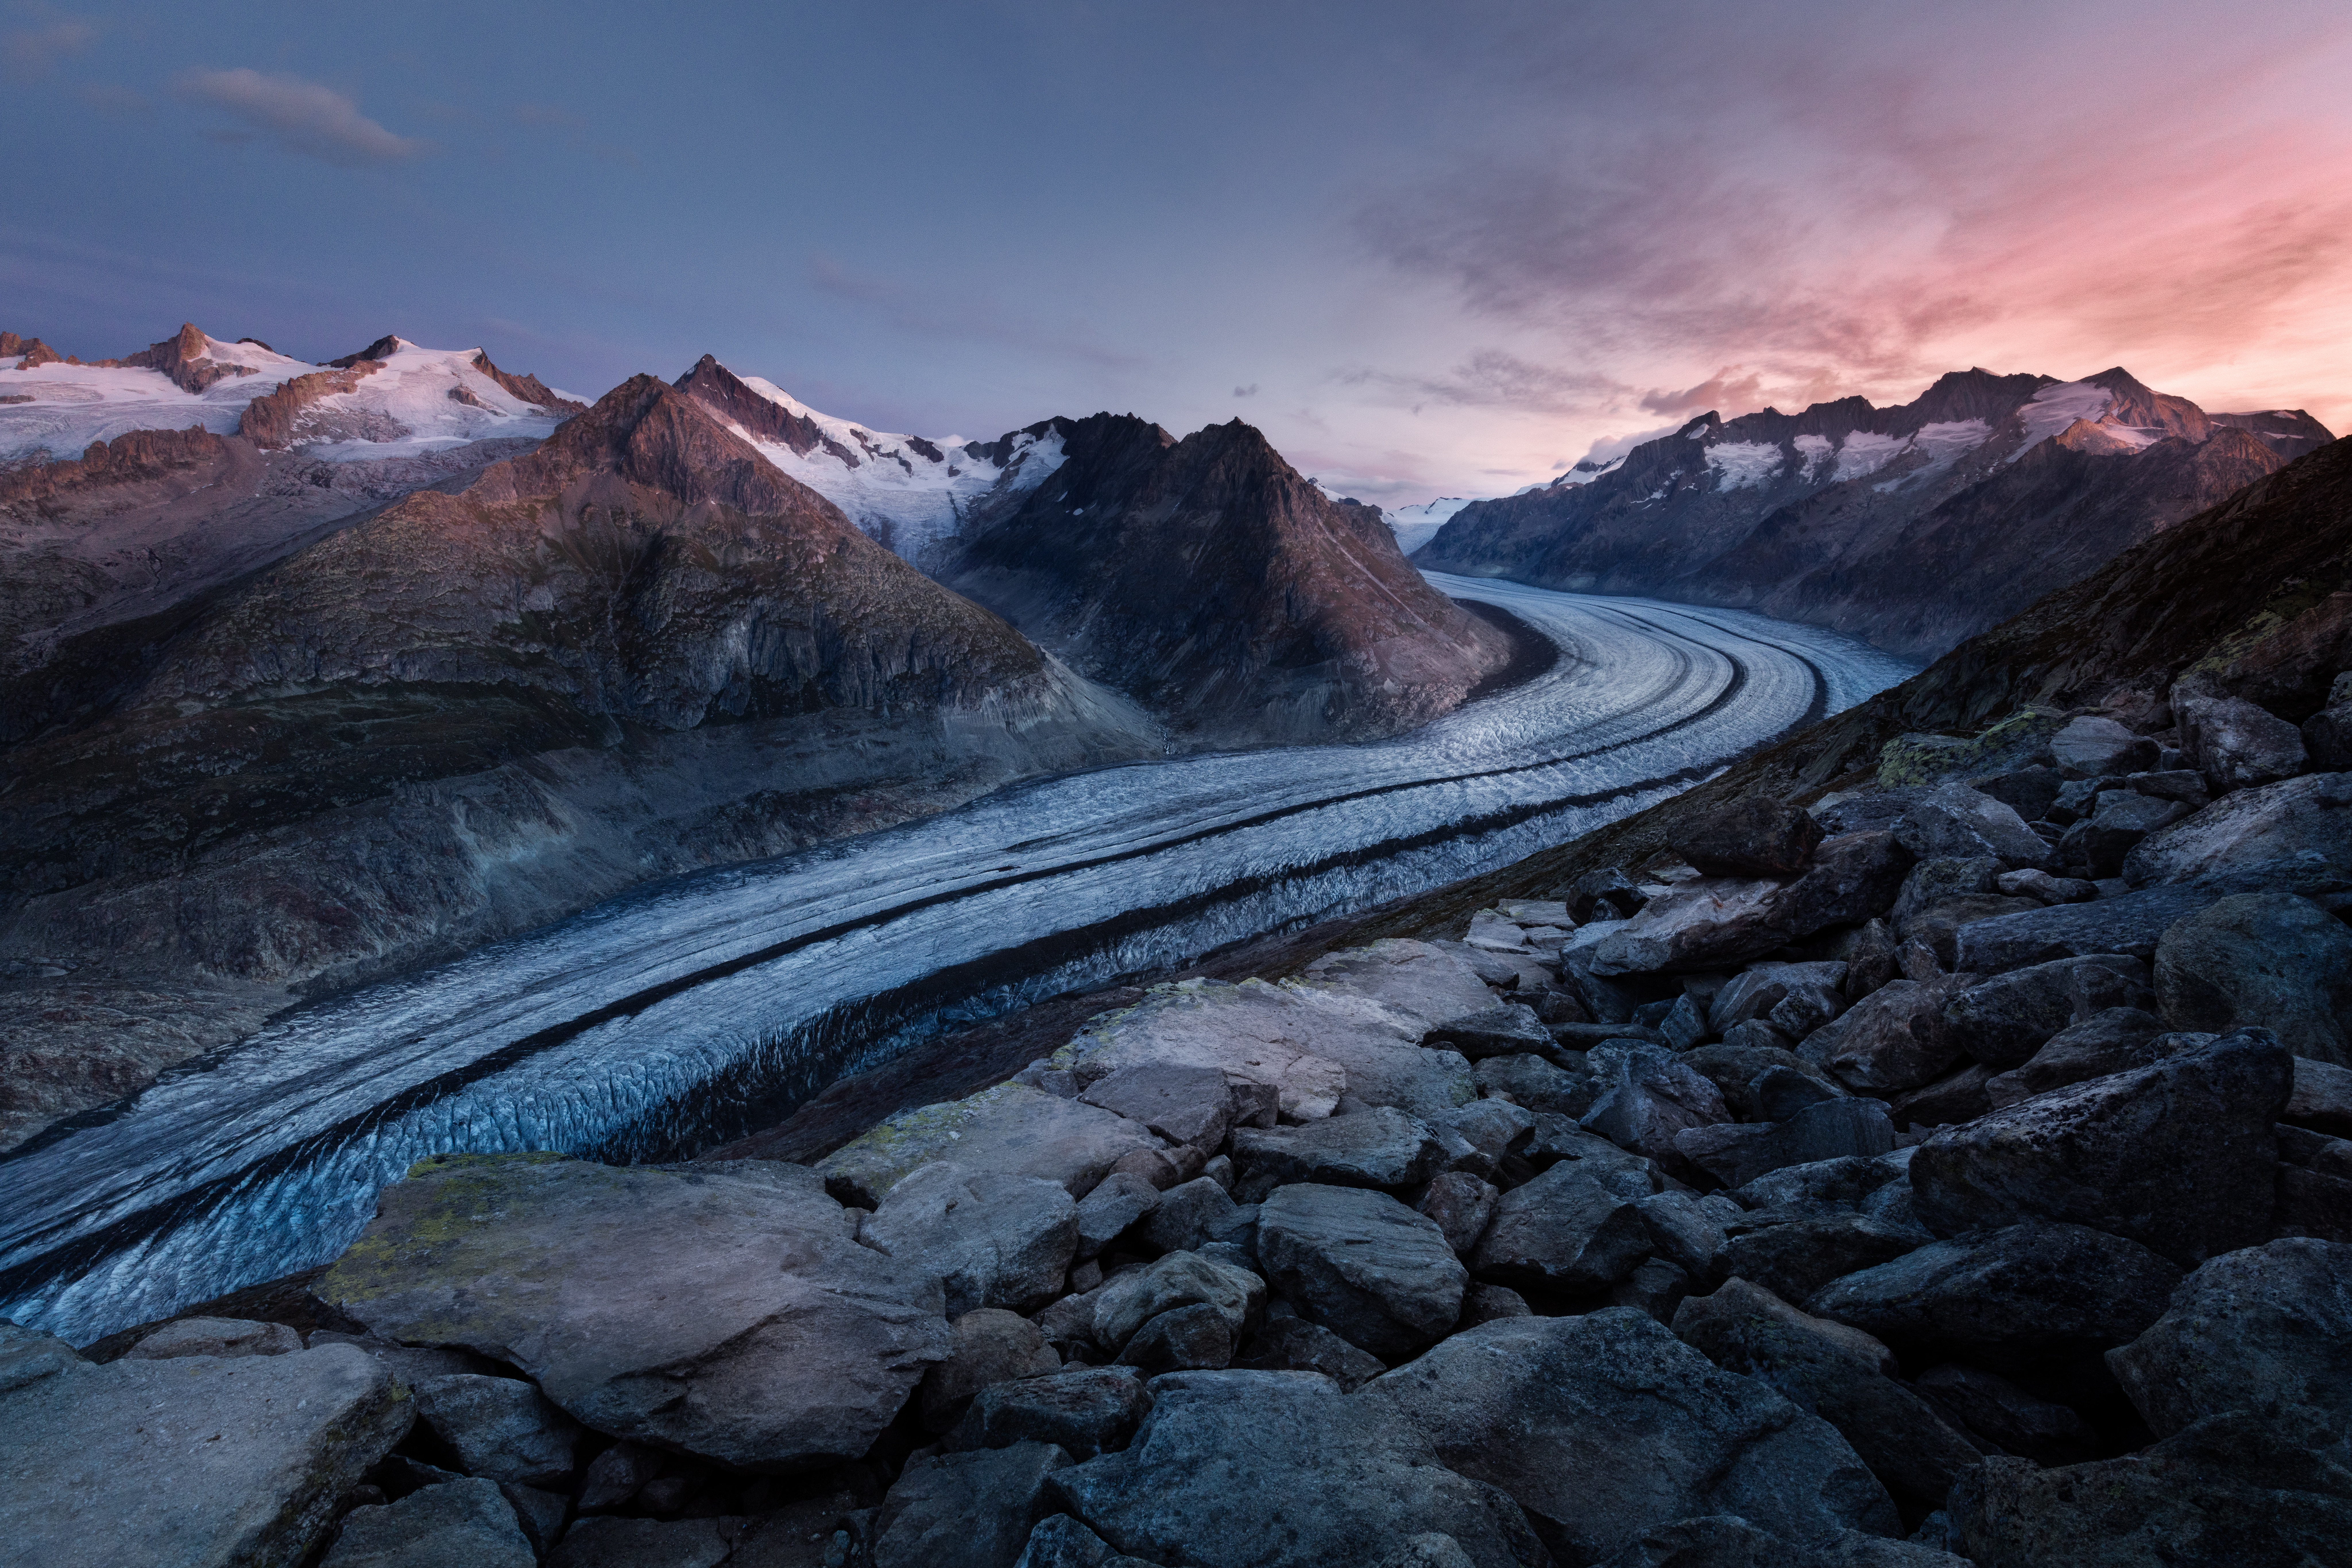
\includegraphics[scale=0.2]{project/images/12.png}
  \caption{\textbf{Administrar Horarios: Jefe de Gestión Escolar}}
\end{figure}
\begin{figure}[H]
  \centering
    \includegraphics[scale=0.2]{project/images/28.png}
  \caption{\textbf{Modificar Horario: Jefe de Gestión Escolar}}
\end{figure}
\begin{figure}[H]
  \centering
    \includegraphics[scale=0.2]{project/images/30.png}
  \caption{\textbf{Habilitar Reinscripción}}
\end{figure}
\begin{figure}[H]
  \centering
    \includegraphics[scale=0.2]{project/images/31.png}
  \caption{\textbf{Cambiar Contraseña}}
\end{figure}
\begin{figure}[H]
  \centering
    \includegraphics[scale=0.15]{project/images/53.png}
  \caption{\textbf{Datos Generales: Académico}}
\end{figure}
\begin{figure}[H]
  \centering
    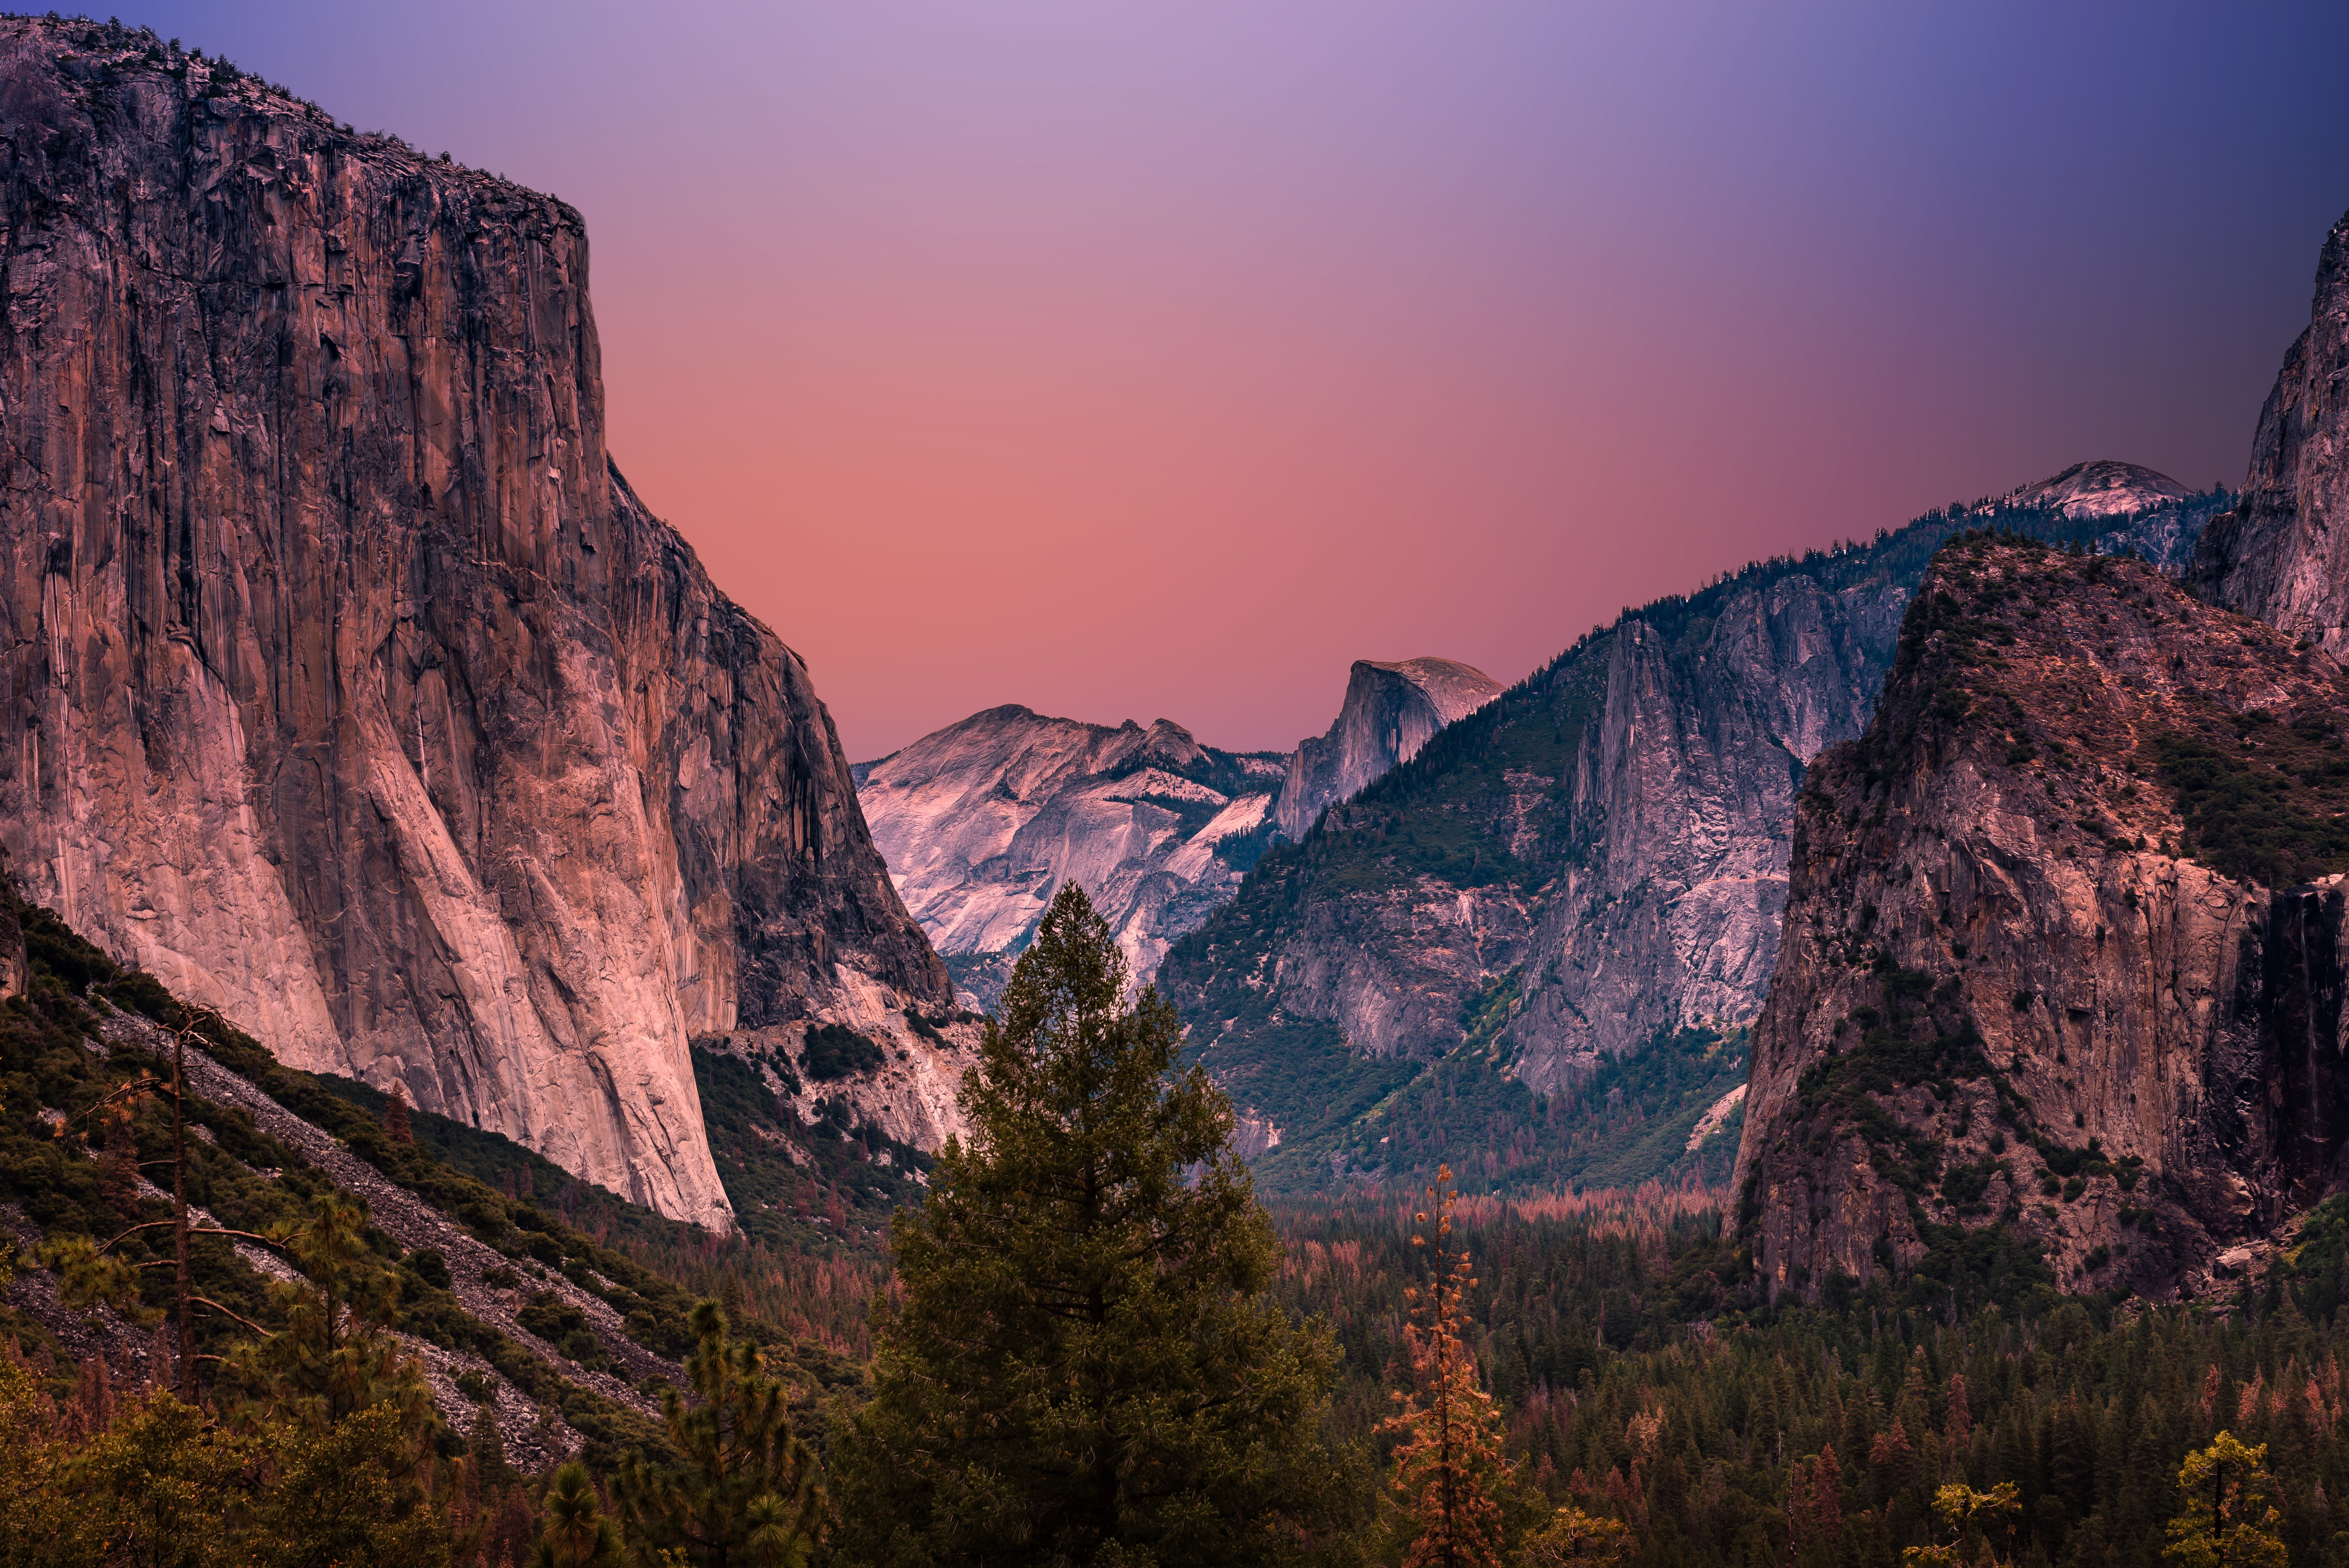
\includegraphics[scale=0.2]{project/images/11.png}
  \caption{\textbf{Asignar Horario: Académico}}
\end{figure}
\begin{figure}[H]
  \centering
    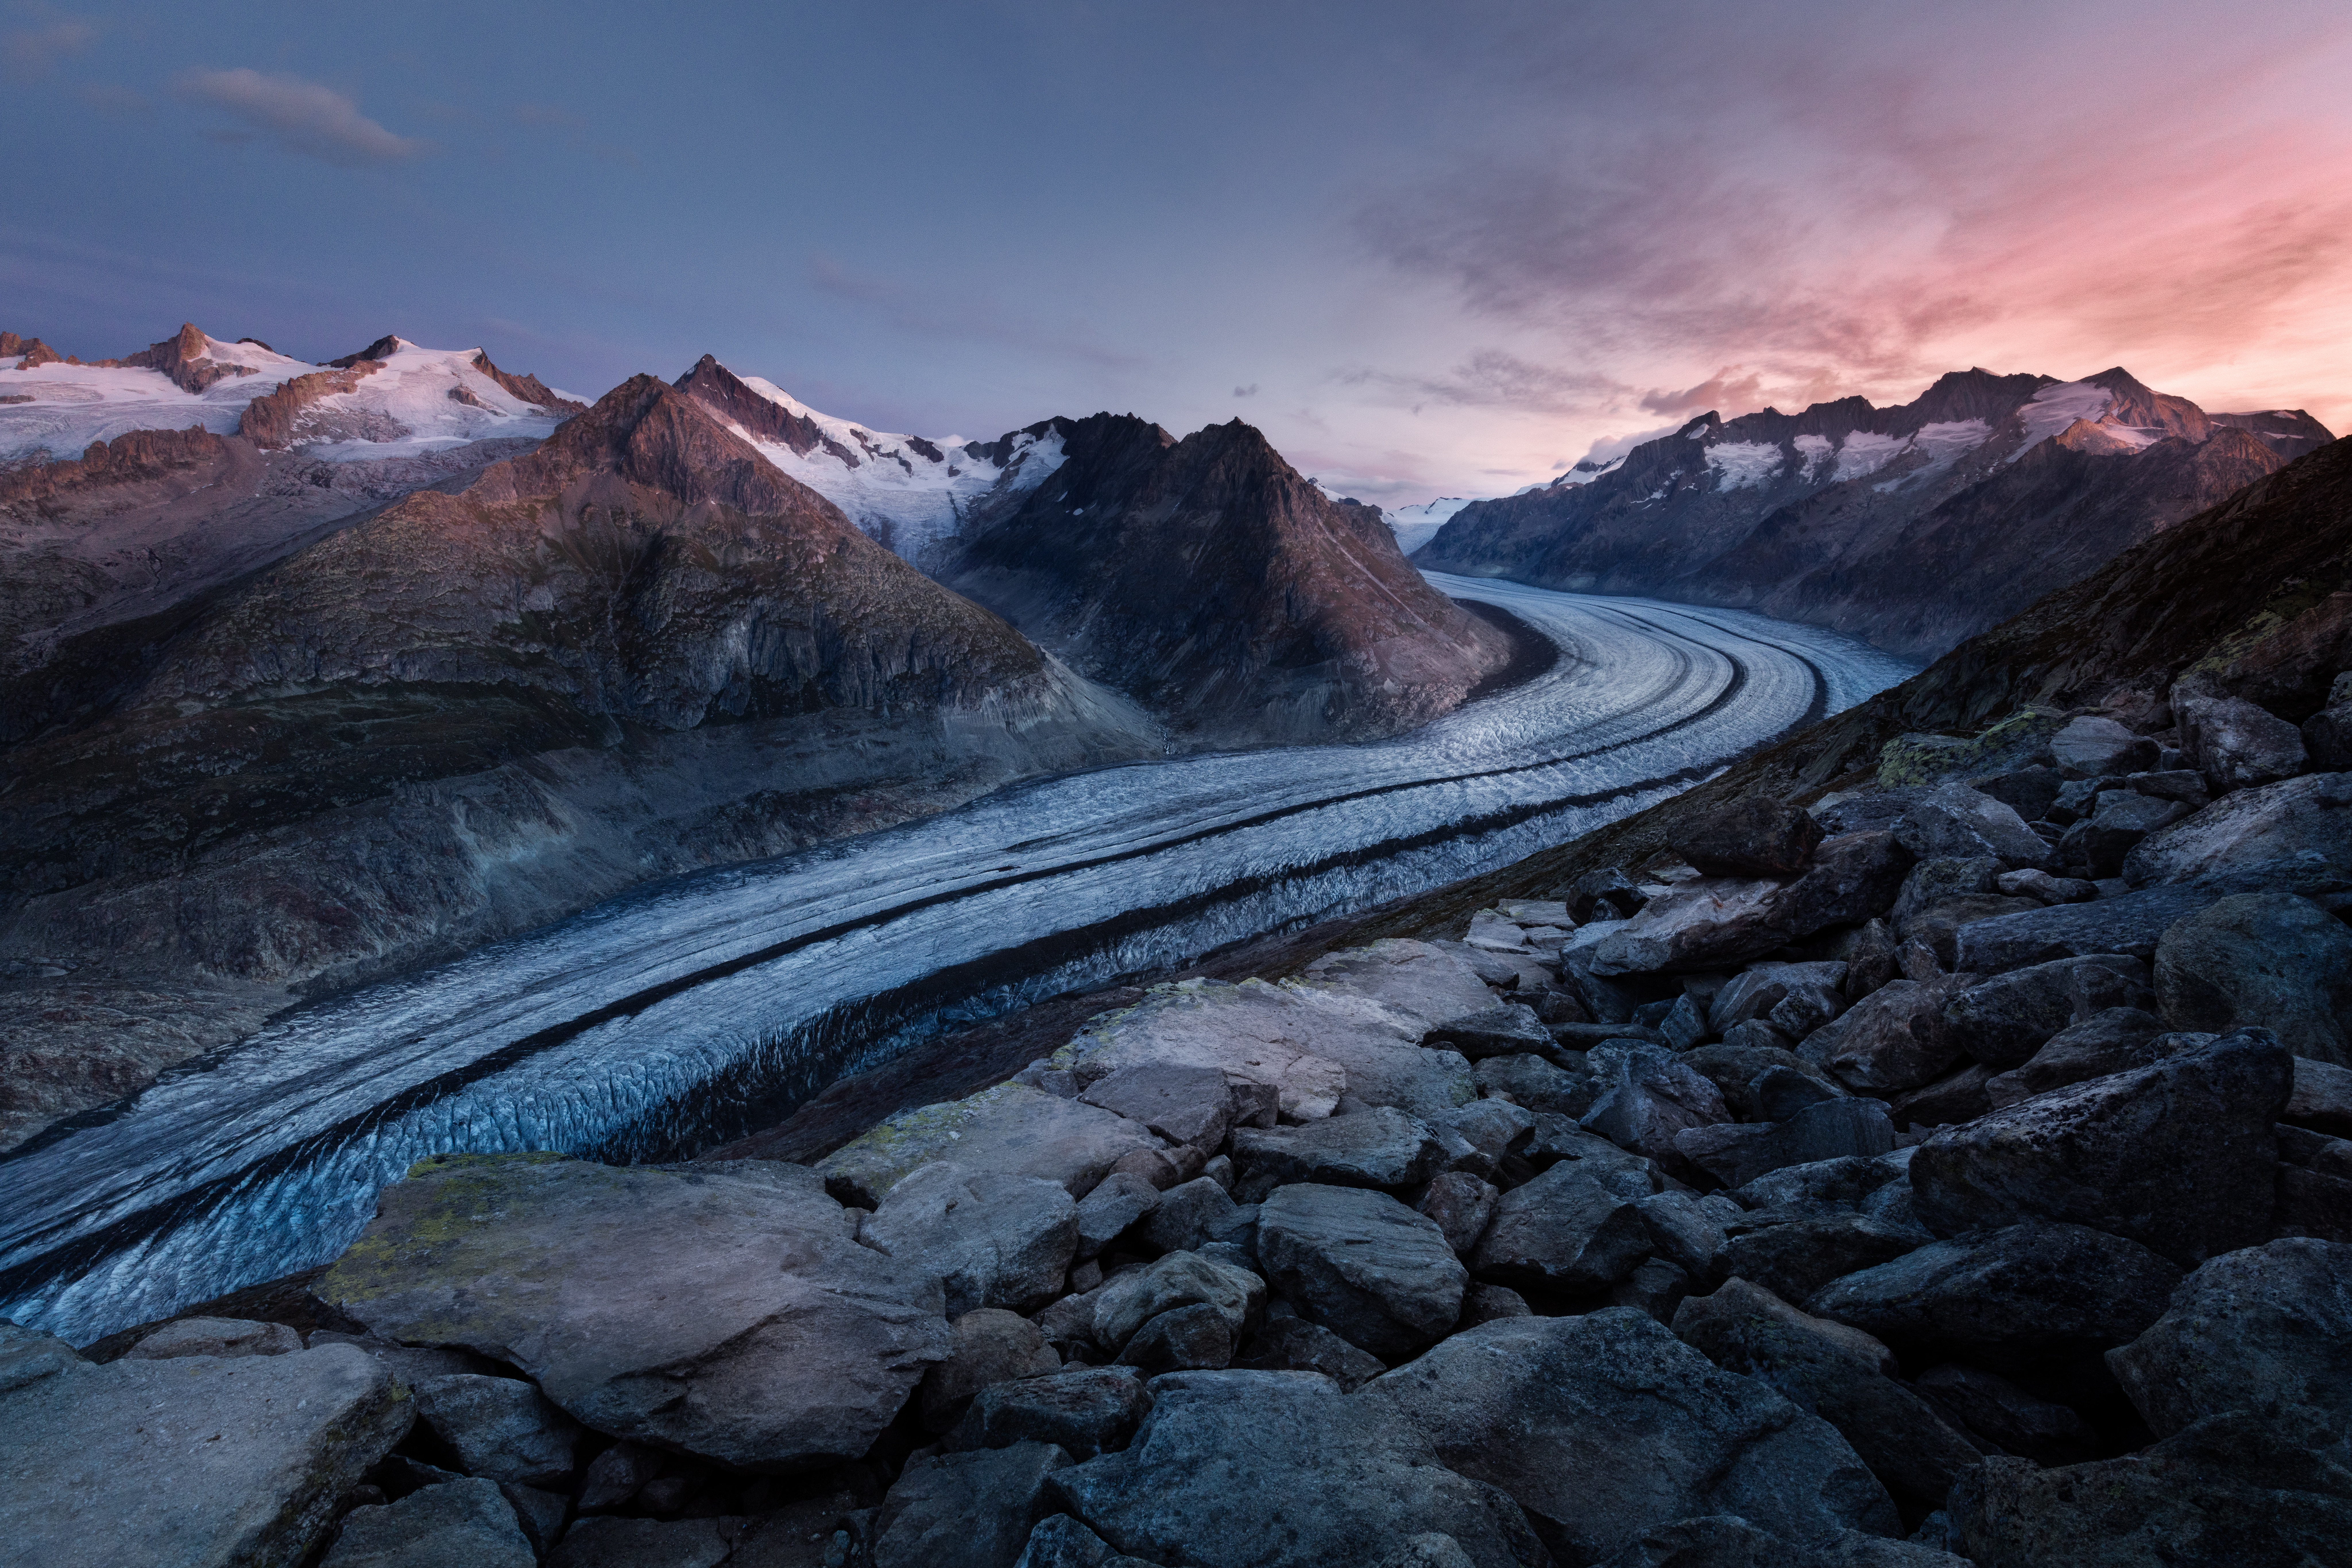
\includegraphics[scale=0.2]{project/images/12.png}
  \caption{\textbf{Administrar Horarios: Académico}}
\end{figure}
\begin{figure}[H]
  \centering
    \includegraphics[scale=0.2]{project/images/13.png}
  \caption{\textbf{Editar Horario: Académico}}
\end{figure}
\begin{figure}[H]
  \centering
    \includegraphics[scale=0.2]{project/images/14.png}
  \caption{\textbf{Cambiar Contraseña}}
\end{figure}
\begin{figure}[H]
  \centering
    \includegraphics[scale=0.15]{project/images/51.png}
  \caption{\textbf{Datos Generales: Analista}}
\end{figure}
\begin{figure}[H]
  \centering
    \includegraphics[scale=0.2]{project/images/36.png}
  \caption{\textbf{Registrar Materia}}
\end{figure}
\begin{figure}[H]
  \centering
    \includegraphics[scale=0.2]{project/images/33.png}
  \caption{\textbf{Registrar Académico: Analista}}
\end{figure}
\begin{figure}[H]
  \centering
    \includegraphics[scale=0.2]{project/images/34.png}
  \caption{\textbf{Registrar Profesor: Analista}}
\end{figure}
\begin{figure}[H]
  \centering
    \includegraphics[scale=0.2]{project/images/35.png}
  \caption{\textbf{Registrar Alumno: Analista}}
\end{figure}
\begin{figure}[H]
  \centering
    \includegraphics[scale=0.2]{project/images/37.png}
  \caption{\textbf{Registrar Grupo}}
\end{figure}
\begin{figure}[H]
  \centering
    \includegraphics[scale=0.2]{project/images/38.png}
  \caption{\textbf{Administrar Académico: Analista}}
\end{figure}
\begin{figure}[H]
  \centering
    \includegraphics[scale=0.2]{project/images/39.png}
  \caption{\textbf{Editar Académico: Analista}}
\end{figure}
\begin{figure}[H]
  \centering
    \includegraphics[scale=0.2]{project/images/40.png}
  \caption{\textbf{Administrar Profesor: Analista}}
\end{figure}
\begin{figure}[H]
  \centering
    \includegraphics[scale=0.2]{project/images/41.png}
  \caption{\textbf{Editar Profesor: Analista}}
\end{figure}
\begin{figure}[H]
  \centering
    \includegraphics[scale=0.2]{project/images/42.png}
  \caption{\textbf{Administrar Alumno: Analista}}
\end{figure}
\begin{figure}[H]
  \centering
    \includegraphics[scale=0.15]{project/images/54.png}
  \caption{\textbf{Editar Alumno: Analista}}
\end{figure}
\begin{figure}[H]
  \centering
    \includegraphics[scale=0.2]{project/images/43.png}
  \caption{\textbf{Administrar Materias}}
\end{figure}
\begin{figure}[H]
  \centering
    \includegraphics[scale=0.2]{project/images/44.png}
  \caption{\textbf{Editar Materia}}
\end{figure}
\begin{figure}[H]
  \centering
    \includegraphics[scale=0.2]{project/images/45.png}
  \caption{\textbf{Administrar Grupo}}
\end{figure}
\begin{figure}[H]
  \centering
    \includegraphics[scale=0.2]{project/images/46.png}
  \caption{\textbf{Editar Grupo}}
\end{figure}
\begin{figure}[H]
  \centering
    \includegraphics[scale=0.2]{project/images/47.png}
  \caption{\textbf{Administrar Tipos de Horario 1}}
\end{figure}
\begin{figure}[H]
  \centering
    \includegraphics[scale=0.2]{project/images/48.png}
  \caption{\textbf{Administrar Tipos de Horario 2}}
\end{figure}
\begin{figure}[H]
  \centering
    \includegraphics[scale=0.2]{project/images/49.png}
  \caption{\textbf{Editar Horario}}
\end{figure}
\begin{figure}[H]
  \centering
    \includegraphics[scale=0.2]{project/images/50.png}
  \caption{\textbf{Cambiar Contraseña}}
\end{figure}
\begin{figure}[H]
  \centering
    \includegraphics[scale=0.2]{project/images/3.png}
  \caption{\textbf{Datos Generales: Alumno}}
\end{figure}
\begin{figure}[H]
  \centering
    \includegraphics[scale=0.2]{project/images/4.png}
  \caption{\textbf{Horario Actual}}
\end{figure}
\begin{figure}[H]
  \centering
    \includegraphics[scale=0.2]{project/images/5.png}
  \caption{\textbf{Disponibilidad y Horarios}}
\end{figure}
\begin{figure}[H]
  \centering
    \includegraphics[scale=0.2]{project/images/6.png}
  \caption{\textbf{Crear Horario 1}}
\end{figure}
\begin{figure}[H]
  \centering
    \includegraphics[scale=0.2]{project/images/7.png}
  \caption{\textbf{Crear Horario 2}}
\end{figure}
\begin{figure}[H]
  \centering
    \includegraphics[scale=0.2]{project/images/8.png}
  \caption{\textbf{Reinscripción}}
\end{figure}
\begin{figure}[H]
  \centering
    \includegraphics[scale=0.2]{project/images/9.png}
  \caption{\textbf{Cambiar Contraseña}}
\end{figure}
\begin{figure}[H]
  \centering
    \includegraphics[scale=0.3]{project/images/editar_horario_alumno_01.jpg}
  \caption{\textbf{Editar Horario de Alumno 1}}
\end{figure}
\begin{figure}[H]
  \centering
    \includegraphics[scale=0.3]{project/images/editar_horario_alumno_02.jpg}
  \caption{\textbf{Editar Horario de Alumno 2}}
\end{figure}
\begin{figure}[H]
  \centering
    \includegraphics[scale=0.3]{project/images/editar_horario_alumno_03.jpg}
  \caption{\textbf{Editar Horario de Alumno 3}}
\end{figure}
\chapter{Diagrama de Casos de Uso}
\begin{figure}[H]
  \centering
    \includegraphics[scale=0.42, angle=90]{project/images/CU.jpg}
\end{figure}
%Aquí solo hay que poner los inputs de los distintos casos de uso, y cada caso de uso manejarlo en un archivo distinto (guardados en la carpeta CU)
\chapter{Descripción de Casos de Uso}
\newpage
\section{Caso de Uso Iniciar Sesión}
\begin{longtable}{ | p{6cm} | p{10cm} |}
	\hline
	\textbf{NOMBRE} & Iniciar Sesión\\
	\hline
	\textbf{TIPO} & Primario\\
	\hline
	\textbf{DESCRIPCIÓN} & El usuario ingresa su ID y su contraseña correspondiente para ingresar al sistema.\\
	\hline
	\textbf{ENTRADAS} & ID de usuario y contraseña.\\
	\hline
	\textbf{SALIDAS} & Mensaje de Error.\\
	\hline
	\textbf{PRECONDICIONES} & Ninguna.\\
	\hline
	\textbf{POSTCONDICIONES} & Ninguna\\
	\hline
	\textbf{SITUACIONES DE ERROR} 
	&
	El ID o contraseña no son correspondientes.\newline
	EL usuario quiere enviar campos vacíos.\newline
	La contraseña no tiene como mínimo 6 caracteres.\\
	\hline
	\textbf{ESTADO DEL SISTEMA EN CASO DE ERROR} & En espera de ingresar el ID correcto y la contraseña correspondiente al ID.\\
	\hline
	\textbf{ACTORES} & Alumno, Jefe de Gestión Escolar (Analista), Analista y Académico.\\
	\hline
	\textbf{MENSAJES} 
	&
	Mensaje de Error ME.31: Extiende este texto para que tenga 6 caracteres o más (actualmente usas <<número de caracteres ingresados>> carácter).\newline
	Mensaje de Error ME.32: El usuario o la contraseña son incorrectos.\newline
	Mensaje de Error ME.37: Completa este campo\\
	\hline
	\textbf{AUTOR} & América Berenice Monsalvo Fuentes\\
	\hline
\end{longtable}
\vspace*{1cm}
\noindent
\Large{PROCEDIMIENTO ESTÁNDAR}
\large{}
\begin{enumerate}
    \item El usuario accede a la vista principal del sistema. (Figura 3.1)
	\item El usuario se dirige a la esquina superior derecha.
	\item El usuario selecciona Iniciar sesión.
	\item *EL sistema muestra el campo Usuario y Contraseña. \textbf{[Trayectoria 3]}
	\item El usuario ingresa su ID de usuario y Contraseña
	\item El usuario selecciona el botón Entrar
	\item *El sistema válida la longitud de la contraseña (al menos 6 caracteres). \textbf{[Trayectoria 1]}
	\item *El sistema busca el ID en la Base de Datos. \textbf{[Trayectoria 2]}
	\item *El sistema válida que la contraseña corresponda al ID y cumpla con el formato con base a RN 2. \textbf{[Trayectoria 2]}
	\item *El sistema direcciona a los Datos generales correspondientes al tipo de usuario. (Figura 3.3)
	\item Fin del caso de uso.
\end{enumerate}
\vspace*{1cm}
\Large{PROCEDIMIENTOS ALTERNATIVOS}\\
	\large{Trayectoria 1}\\
	\textbf{Condición:} El ID no existe en la Base de Datos.
	\begin{enumerate}
		\item *El sistema muestra el Mensaje de Error ME.1.
		\item *Se vuelve al punto 5 de la trayectoria principal.
		\item Fin de la trayectoria
	\end{enumerate}
	\large{Trayectoria 2}\\
	\textbf{Condición:} La contraseña no corresponde al ID.
	\begin{enumerate}
		\item *El sistema muestra el Mensaje de Error ME.32.
		\item *El sistema limpia todos los campos.
		\item *Se vuelve al punto 5 de la trayectoria principal
		\item Fin de la trayectoria
	\end{enumerate}
	\large{Trayectoria 3}\\
	\textbf{Condición:} Selecciona el botón entrar sin llenar los campo mostrados.
	\begin{enumerate}
		\item *El sistema muestra el Mensaje de Error ME.37.
		\item *Se vuelve al punto 5 de la trayectoria principal
		\item Fin de la trayectoria
	\end{enumerate}
\newpage
\section{Caso de Uso Registrar Alumno}
\begin{longtable}{ | p{6cm} | p{10cm} |}
\hline
\textbf{NOMBRE} & Registrar Alumno\\
\hline
\textbf{TIPO} & Primario\\
\hline
\textbf{DESCRIPCIÓN} & El analista registra los datos del alumno en un formulario otorgandole un perfil en el sistema.\\
\hline
\textbf{ENTRADAS} & Nombre del alumno: Caracteres (solo letras)\\& Apellido Paterno: Caracteres (solo letras)\\& Apellido Materno: Caracteres (solo letras)\\&Número de Boleta: Números con longitud de 10 dígitos\\& Correo Electrónico: Caracteres con el formato de correo electrónico\\& Contraseña: longitud de 6 a 20 caracteres.\\
\hline
\textbf{SALIDAS} & Se mostrará un mensaje de confirmación si el registro fue exitoso.\\& Se mostrará un mensaje de error cuando falten campos por llenar o el formato no sea correcto.\\
\hline
\textbf{PRECONDICIONES} & No hay\\
\hline
\textbf{POSTCONDICIONES} & Se registran los datos del alumno en la base de datos y se le otorga una cuenta\\
\hline
\textbf{SITUACIONES DE ERROR} & \begin{itemize}
    \item Se dejaron campos obligatorios en blanco.
    \item El correo ya ha sido registrado en otra cuenta.
    \item El formato de los datos es inválido.
    \item El número de boleta ya fue asignado a otro alumno.
\end{itemize}\\
\hline
\textbf{ESTADO DEL SISTEMA EN CASO DE ERROR} & No se registran los datos del alumno\\
\hline
\textbf{ACTORES} & Analista, Jefe de Gestión Escolar\\
\hline
\textbf{MENSAJES} & \textbf{Mensaje de Confirmación}: Se muestra cuando los datos han sido almacenados correctamente: MC.1\\&\textbf{Mensajes de Error}: Se muestran en los siguientes casos:\begin{itemize}
    \item Se dejaron campos obligatorios en blanco: ME.1
    \item El formato de los datos es inválido: ME.2
    \item El correo está registrado en otra cuenta: ME.3
    \item El número de boleta ya fue asignado a otro alumno: ME.4
\end{itemize}\\
\hline
\textbf{AUTOR} & Hernández Pineda Miguel Angel\\
\hline
\end{longtable}
\vspace*{1cm}
\noindent
\Large{PROCEDIMIENTO ESTÁNDAR}
\large{}
\begin{enumerate}
    \item El usuario ingresa al sistema como Analista o Jefe de Gestión Escolar.
    \item El usuario da click en la opción de <<Registrar Alumno>> de la sección Registrar (Figura 3.14)
    \item El usuario ingresa el nombre del alumno.
    \item El usuario ingresa el apellido paterno.
    \item El usuario ingresa el apellido materno.
    \item El usuario ingresa el número de boleta.
    \item El usuario ingresa el correo electrónico.
    \item El usuario ingresa la contraseña del alumno.
    \item El usuario da click en el botón enviar.
    \item El sistema valida que no haya campos obligatorios en blanco. \textbf{[Trayectoria 1]}
    \item *El sistema valida los datos en el campo de nombre. \textbf{[Trayectoria 2]}
    \item *El sistema valida los datos en el campo de apellido paterno. \textbf{[Trayectoria 3]}
    \item *El sistema valida los datos en el campo de apellido materno. \textbf{[Trayectoria 4]}
    \item *El sistema valida los datos en el campo de número de boleta. \textbf{[Trayectoria 5]} \textbf{[Trayectoria 6]}
    \item *El sistema valida los datos en el campo de correo electrónico. \textbf{[Trayectoria 7]} \textbf{[Trayectoria 8]}
    \item *El sistema valida los datos en el campo de contraseña según la regla de negocio RN.2. \textbf{[Trayectoria 9]}
    \item Se registran los datos del alumno y se crea un perfil en el sistema.
    \item Se muestra un mensaje de confirmación MC.1.
    \item Fin del caso de uso
\end{enumerate}
\vspace*{1cm}
\Large{PROCEDIMIENTOS ALTERNATIVOS}\\
\large{Trayectoria 1}\\
\textbf{Condición}: Quedaron campos obligatorios en blanco.
\begin{enumerate}
    \item *El sistema muestra el mensaje de error ME.1.
    \item *El sistema marca de color rojo los campos vacios.
    \item Regresa al punto 3 de la trayectoria principal.
    \item Fin de la trayectoria.
\end{enumerate}
\large{Trayectoria 2}\\
\textbf{Condición}: El formato de texto para el campo nombre del alumno es inválido.
\begin{enumerate}
    \item *El sistema muestra el mensaje de error ME.2.
    \item *El sistema marca de color rojo el campo de nombre.
    \item Regresa al punto 3 de la trayectoria principal.
    \item Fin de la trayectoria.
\end{enumerate}
\large{Trayectoria 3}\\
\textbf{Condición}: El formato de texto para el campo apellido paterno es inválido.
\begin{enumerate}
    \item *El sistema muestra el mensaje de error ME.2.
    \item *El sistema marca de color rojo el campo de apellido paterno.
    \item Regresa al punto 4 de la trayectoria principal.
    \item Fin de la trayectoria.
\end{enumerate}
\large{Trayectoria 4}\\
\textbf{Condición}: El formato de texto para el campo apellido materno es inválido.
\begin{enumerate}
    \item *El sistema muestra el mensaje de error ME.2.
    \item *El sistema marca de color rojo el campo de apellido materno.
    \item Regresa al punto 5 de la trayectoria principal.
    \item Fin de la trayectoria.
\end{enumerate}
\large{Trayectoria 5}\\
\textbf{Condición}: El formato de los datos en el campo número de boleta es inválido.
\begin{enumerate}
    \item *El sistema muestra el mensaje de error ME.2.
    \item *El sistema marca de color rojo el campo número de boleta.
    \item Regresa al punto 6 de la trayectoria principal.
    \item Fin de la trayectoria.
\end{enumerate}
\large{Trayectoria 7}\\
\textbf{Condición}: El número de boleta ingresado ya ha sido asignado a otro alumno.
\begin{enumerate}
    \item *El sistema muestra el mensaje de error ME.4.
    \item *El sistema marca de color rojo el campo número de boleta.
    \item Regresa al punto 6 de la trayectoria principal.
    \item Fin de la trayectoria.
\end{enumerate}
\large{Trayectoria 7}\\
\textbf{Condición}: El formato del correo electrónico es inválido.
\begin{enumerate}
    \item *El sistema muestra el mensaje de error ME.2.
    \item *El sistema marca de color rojo el campo de correo electrónico.
    \item Regresa al punto 7 de la trayectoria principal.
    \item Fin de la trayectoria.
\end{enumerate}
\large{Trayectoria 8}\\
\textbf{Condición}: El correo electrónico ingresado ya fue registrado en otra cuenta.
\begin{enumerate}
    \item *El sistema muestra el mensaje de error ME.3.
    \item *El sistema marca de color rojo el campo de correo electrónico.
    \item Regresa al punto 7 de la trayectoria principal.
    \item Fin de la trayectoria.
\end{enumerate}
\large{Trayectoria 9}\\
\textbf{Condición}: El formato de la contraseña es inválido según la regla de negocio RN.2.
\begin{enumerate}
    \item *El sistema muestra el mensaje de error ME.2.
    \item *El sistema marca de color rojo el campo de contraseña.
    \item Regresa al punto 8 de la trayectoria principal.
    \item Fin de la trayectoria.
\end{enumerate}
\newpage
\section{Caso de Uso Registrar Académico}
\begin{longtable}{ | p{6cm} | p{10cm} |}
\hline
\textbf{NOMBRE} & Registrar Académico\\
\hline
\textbf{TIPO} & Primario\\
\hline
\textbf{DESCRIPCIÓN} & El usuario registra los datos del Académico en un formulario otorgandole un perfil en el sistema.\\
\hline
\textbf{ENTRADAS} & Nombre del Académico: Caracteres (solo letras)\\& Apellido Paterno: Caracteres (solo letras)\\& Apellido Materno: Caracteres (solo letras)\\&Número de empleado: Números con longitud de 10 dígitos\\&RFC: Números y letras con el formato de RFC con longitud de 10 dígitos\\& Correo Electrónico: Caracteres con el formato de correo electrónico\\& Contraseña: longitud de 6 a 20 caracteres.\\
\hline
\textbf{SALIDAS} & Se mostrará un mensaje de confirmación si el registro fue exitoso.\\& Se mostrará un mensaje de error cuando falten campos por llenar o el formato no sea correcto.\\
\hline
\textbf{PRECONDICIONES} & No hay\\
\hline
\textbf{POSTCONDICIONES} & Se registran los datos del Académico en la base de datos y se le otorga una cuenta\\
\hline
\textbf{SITUACIONES DE ERROR} & \begin{itemize}
    \item Se dejaron campos obligatorios en blanco.
    \item El correo ya ha sido registrado en otra cuenta.
    \item El formato de los datos es inválido.
    \item El número de empleado ya fue asignado a otro Académico.
\end{itemize}\\
\hline
\textbf{ESTADO DEL SISTEMA EN CASO DE ERROR} & No se registran los datos del Académico\\
\hline
\textbf{ACTORES} & Analista, Jefe de Gestión Escolar\\
\hline
\end{longtable}
\newpage
\begin{longtable}{ | p{6cm} | p{10cm} |}
\hline
\textbf{MENSAJES} & \textbf{Mensaje de Confirmación}: Se muestra cuando los datos han sido almacenados correctamente: MC.1\\&\textbf{Mensajes de Error}: Se muestran en los siguientes casos:\begin{itemize}
    \item Se dejaron campos obligatorios en blanco: ME.1
    \item El formato de los datos es inválido: ME.2
    \item El correo está registrado en otra cuenta: ME.3
    \item El número de empleado ya fue asignado a otro Académico: ME.5
\end{itemize}\\
\hline
\textbf{AUTOR} & Matus López Carlos Eduardo\\
\hline
\end{longtable}
\vspace*{1cm}
\noindent
\Large{PROCEDIMIENTO ESTÁNDAR}
\large{}
\begin{enumerate}
    \item El usuario ingresa al sistema como Analista o Jefe de Gestión Escolar.
    \item El usuario da click en la opción de <<Registrar Académico>> de la sección Registrar (Figura 3.14)
    \item El usuario ingresa el nombre del profesor.
    \item El usuario ingresa el apellido paterno.
    \item El usuario ingresa el apellido materno.
    \item El usuario ingresa el número de empleado.
    \item El usuario ingresa el correo electrónico.
    \item El usuario ingresa el RFC del profesor.
    \item El usuario ingresa la contraseña del profesor.
    \item El usuario da click en el botón enviar.
    \item El sistema valida que no haya campos obligatorios en blanco. \textbf{[Trayectoria 1]}
    \item *El sistema valida los datos en el campo de nombre. \textbf{[Trayectoria 2]}
    \item *El sistema valida los datos en el campo de apellido paterno. \textbf{[Trayectoria 3]}
    \item *El sistema valida los datos en el campo de apellido materno. \textbf{[Trayectoria 4]}
    \item *El sistema valida los datos en el campo de número de empleado. \textbf{[Trayectoria 5]} \textbf{[Trayectoria 9]}
    \item *El sistema valida los datos en el campo de correo electrónico. \textbf{[Trayectoria 6]}
    \item *El sistema valida los datos en el campo de RFC. \textbf{[Trayectoria 7]}
    \item *El sistema valida los datos en el campo de contraseña según la regla de negocio RN.2. \textbf{[Trayectoria 8]}
    \item Se registran los datos del profesor y se crea un perfil en el sistema.
    \item Se muestra un mensaje de confirmación MC.1.
    \item Fin del caso de uso
\end{enumerate}
\vspace*{1cm}
\Large{PROCEDIMIENTOS ALTERNATIVOS}\\
\large{Trayectoria 1}\\
\textbf{Condición}: Quedaron campos obligatorios en blanco.
\begin{enumerate}
    \item *El sistema muestra el mensaje de error ME.1.
    \item *El sistema marca de color rojo los campos vacios.
    \item Regresa al punto 3 de la trayectoria principal.
    \item Fin de la trayectoria.
\end{enumerate}
\large{Trayectoria 2}\\
\textbf{Condición}: El formato de texto para el campo nombre del alumno es inválido.
\begin{enumerate}
    \item *El sistema muestra el mensaje de error ME.2.
    \item *El sistema marca de color rojo el campo de nombre.
    \item Regresa al punto 3 de la trayectoria principal.
    \item Fin de la trayectoria.
\end{enumerate}
\large{Trayectoria 3}\\
\textbf{Condición}: El formato de texto para el campo apellido paterno es inválido.
\begin{enumerate}
    \item *El sistema muestra el mensaje de error ME.2.
    \item *El sistema marca de color rojo el campo de apellido paterno.
    \item Regresa al punto 4 de la trayectoria principal.
    \item Fin de la trayectoria.
\end{enumerate}
\large{Trayectoria 4}\\
\textbf{Condición}: El formato de texto para el campo apellido materno es inválido.
\begin{enumerate}
    \item *El sistema muestra el mensaje de error ME.2.
    \item *El sistema marca de color rojo el campo de apellido materno.
    \item Regresa al punto 5 de la trayectoria principal.
    \item Fin de la trayectoria.
\end{enumerate}
\large{Trayectoria 5}\\
\textbf{Condición}: El formato de los datos en el campo número de empleado es inválido.
\begin{enumerate}
    \item *El sistema muestra el mensaje de error ME.2.
    \item *El sistema marca de color rojo el campo número de empleado.
    \item Regresa al punto 6 de la trayectoria principal.
    \item Fin de la trayectoria.
\end{enumerate}
\large{Trayectoria 6}\\
\textbf{Condición}: El formato del correo electrónico es inválido.
\begin{enumerate}
    \item *El sistema muestra el mensaje de error ME.2.
    \item *El sistema marca de color rojo el campo de correo electrónico.
    \item Regresa al punto 7 de la trayectoria principal.
    \item Fin de la trayectoria.
\end{enumerate}
\large{Trayectoria 7}\\
\textbf{Condición}: El formato del RFC es inválido.
\begin{enumerate}
    \item *El sistema muestra el mensaje de error ME.2.
    \item *El sistema marca de color rojo el campo de RFC.
    \item Regresa al punto 8 de la trayectoria principal.
    \item Fin de la trayectoria.
\end{enumerate}
\large{Trayectoria 8}\\
\textbf{Condición}: El formato de la contraseña es inválido según la regla de negocio RN.2.
\begin{enumerate}
    \item *El sistema muestra el mensaje de error ME.2.
    \item *El sistema marca de color rojo el campo de contraseña.
    \item Regresa al punto 9 de la trayectoria principal.
    \item Fin de la trayectoria.
\end{enumerate}
\large{Trayectoria 9}\\
\textbf{Condición}: El número de empleado asignado ya ha sido registrado.
\begin{enumerate}
    \item *El sistema muestra el mensaje de error ME.5.
    \item *El sistema marca de color rojo el campo número de empleado.
    \item Regresa al punto 6 de la trayectoria principal.
    \item Fin de la trayectoria.
\end{enumerate}
\newpage
\section{Caso de Uso Registrar Materia}
\begin{longtable}{ | p{6cm} | p{10cm} |}
\hline
\textbf{NOMBRE} & Registrar Materia\\
\hline
\textbf{TIPO} & Primario\\
\hline
\textbf{DESCRIPCIÓN} & El analista registra los datos de una nueva unidad de aprendizaje\\
\hline
\textbf{ENTRADAS} & Nombre de la Materia: Cadena de caracteres\\ & Créditos: Valor numérico con dos decimales\\ & Nivel: Selección de una lista numérica (entre 1 y 4)\\ & Área: Selección de área de una lista.\\ & Cupo: Selección de una lista numérica (entre 25 y 35)\\
\hline
\textbf{SALIDAS} & Se mostrará un mensaje de confirmación si los datos se registran de manera exitosa.\\ & Se mostrará un mensaje de error si se dejaron campos en blanco, o el formato de los datos no es correcto.\\
\hline
\textbf{PRECONDICIONES} & No hay\\
\hline
\textbf{POSTCONDICIONES} & Se registra una nueva materia dentro del mapa curricular.\\
\hline
\textbf{SITUACIONES DE ERROR} & \begin{itemize}
    \item Se dejaron campos obligatorios en blanco.
    \item El formato de los datos es inválido.
\end{itemize}\\
\hline
\textbf{ESTADO DEL SISTEMA EN CASO DE ERROR} & No se registra la materia.\\
\hline
\textbf{ACTORES} & Analista\\
\hline
\textbf{MENSAJES} & \textbf{Mensaje de Confirmación}: Se muestra cuando los datos han sido almacenados correctamente: MC.1\\ & \textbf{Mensajes de Error}: Se muestran en los siguientes casos: \begin{itemize}
    \item Se dejaron campos obligatorios en blanco: ME.1
    \item El formato de los datos es inválido: ME.2
\end{itemize}\\
\hline
\textbf{AUTOR} & Hernández Pineda Miguel Angel\\
\hline
\end{longtable}
\newpage
\noindent
\Large{PROCEDIMIENTO ESTÁNDAR}
\large{}
\begin{enumerate}
    \item El usuario ingresa al sistema como Analista.
    \item El usuario da click en la opción <<Registrar Materia>> de la Sección Registrar (Figura 3.15)
    \item El usuario ingresa el nombre de la materia.
    \item El usuario ingresa el número de créditos de la materia.
    \item El usuario selecciona un nivel.
    \item El usuario selecciona un área de conocimiento.
    \item El usuario da click en el botón enviar.
    \item *El sistema valida que no haya campos obligatorios en blanco. \textbf{[Trayectoria 1]}
    \item *El sistema valida los datos en el campo de nombre de la materia. \textbf{[Trayectoria 2]}
    \item *El sistema valida los datos en el campo de créditos según la regla de negocio RN.15. \textbf{[Trayectoria 3]}
    \item Se registra la materia de forma correcta en el mapa curricular.
    \item Se muestra el mensaje de confirmación MC.1.
    \item Fin del caso de uso.
\end{enumerate}
\vspace*{1cm}
\Large{PROCEDIMIENTOS ALTERNATIVOS}\\
\large{Trayectoria 1}\\
\textbf{Condición}: Se dejaron campos obligatorios en blanco.
\begin{enumerate}
    \item *El sistema muestra el mensaje de error ME.1.
    \item *El sistema marca de color rojo los campos vacíos.
    \item Regresa al punto 3 de la trayectoria principal.
    \item Fin de la trayectoria.
\end{enumerate}
\large{Trayectoria 2}\\
\textbf{Condición}: El formato de texto para el campo de nombre de la materia es inválido.
\begin{enumerate}
    \item *El sistema muestra el mensaje de error ME.2.
    \item *El sistema marca de color rojo el campo de nombre.
    \item Regresa al punto 3 de la trayectoria principal.
    \item Fin de la trayectoria.
\end{enumerate}
\large{Trayectoria 3}\\
\textbf{Condición}: El formato para el campo de créditos es inválido según la regla de negocio RN.15.
\begin{enumerate}
    \item *El sistema muestra el mensaje de error ME.2.
    \item *El sistema marca de color rojo el campo de créditos.
    \item Regresa al punto 4 de la trayectoria principal.
    \item Fin de la trayectoria.
\end{enumerate}
\input{project/CU/registrar_profesor.tex}
\newpage
\section{Prueba P8: Caso de Uso Generar Grupo}
\begin{longtable}{ | p{9cm} | p{.5cm} | p{.5cm} | p{5cm} | }
\hline
\textbf{Pregunta} & \textbf{Si} & \textbf{No} & \textbf{Observaciones}\\
\hline
\multicolumn{4}{| p{15cm}| }{1. Inicie sesión en el sistema como un jefe de gestión escolar con los siguientes datos: \begin{itemize}
\item Usuario: \textbf{MOMM710615GH1}
\item Contraseña: \textbf{Mar1sol}
\end{itemize}
2. En el menú izquierdo seleccione la opción <<Registro>> y posteriormente de clic en <<Registrar Grupo>>. \newline
3. En la pantalla Horario Actual envíe el formulario con los campos vacíos al darle clic en Registrar Grupo.
}\\
\hline
3.1  ¿El sistema evitó el registro de un nuevo grupo? & & &\\
\hline
3.2  ¿El sistema mostró correctamente el error ME.1? & & &\\
\hline
\textbf{Pregunta} & \textbf{Si} & \textbf{No} & \textbf{Observaciones}\\
\hline
\multicolumn{4}{| p{15cm}| }{4. Ingrese ahora los siguientes datos:  \begin{itemize}
\item Turno: \textbf{Matutino}
\item Nivel del grupo: \textbf{1}
\item Número del grupo: \textbf{1}
\end{itemize}
}\\
\hline
4.1  ¿El sistema evitó el registro de un nuevo grupo? & & &\\
\hline
4.2  ¿El sistema mostró correctamente el error ME.33? & & &\\
\hline
\textbf{Pregunta} & \textbf{Si} & \textbf{No} & \textbf{Observaciones}\\
\hline
\multicolumn{4}{| p{15cm}| }{5. Ingrese ahora los siguientes datos:  \begin{itemize}
\item Turno: \textbf{Vespertino}
\item Nivel del grupo: \textbf{1}
\item Número del grupo: \textbf{1}
\end{itemize}
}\\
\hline
5.1  ¿El sistema mostró correctamente la MC.1? & & &\\
\hline
\multicolumn{4}{| p{15cm}| }{\textbf{Fin de la Prueba}} \\
\hline
\end{longtable}
\input{project/CU/registrar_grupo.tex}
\newpage
\section{Caso de Uso Modificar Alumno}
\begin{longtable}{ | p{6cm} | p{10cm} |}
\hline
\textbf{NOMBRE} & Modificar Alumno\\
\hline
\textbf{TIPO} & Secundario\\
\hline
\textbf{DESCRIPCIÓN} & El usuario modifica los datos del alumno en un formulario.\\
\hline
\textbf{ENTRADAS} & Nombre del alumno: Caracteres (solo letras)\\& Apellido Paterno: Caracteres (solo letras)\\& Apellido Materno: Caracteres (solo letras)\\&Número de Boleta: Números con longitud de 10 dígitos\\& Correo Electrónico: Caracteres con el formato de correo electrónico\\& Contraseña: longitud de 6 a 20 caracteres.\\
\hline
\textbf{SALIDAS} & Se mostrará un mensaje de confirmación si la modificacion del registro fue exitosa.\\& Se mostrará un mensaje de error cuando falten campos por llenar o el formato no sea correcto.\\
\hline
\textbf{PRECONDICIONES} & Registro de alumnos previamente \\
\hline
\textbf{POSTCONDICIONES} & Se modifican los datos del alumno en la base de datos  \\
\hline
\textbf{SITUACIONES DE ERROR} & \begin{itemize}
   \item  No hay alumnos registrados
    \item Se dejaron campos obligatorios en blanco.
    \item El correo ya ha sido registrado en otra cuenta.
    \item El formato de los datos es inválido.
    \item El número de boleta ya fue asignado a otro alumno.
\end{itemize}\\
\hline
\textbf{ESTADO DEL SISTEMA EN CASO DE ERROR} & No se modifican los datos del alumno\\
\hline
\textbf{ACTORES} & Analista, Jefe de Gestión Escolar\\
\hline
\textbf{MENSAJES} & \textbf{Mensaje de Confirmación}: Se muestra cuando los datos han sido modificados correctamente: MC.2\\&\textbf{Mensajes de Error}: Se muestran en los siguientes casos:\begin{itemize}
\item No hay alumnos registrados ME.17
    \item Se dejaron campos obligatorios en blanco: ME.1
    \item El formato de los datos es inválido: ME.2
    \item El correo está registrado en otra cuenta: ME.3
    \item El número de boleta ya fue asignado a otro alumno: ME.4
\end{itemize}\\
\hline
\textbf{AUTOR} & Matus López Carlos Eduardo\\
\hline
\end{longtable}
\vspace*{1cm}
\noindent
\Large{PROCEDIMIENTO ESTÁNDAR}
\large{}
\begin{enumerate}
    \item El usuario ingresa al sistema como Analista o Jefe de Gestión Escolar.
    \item El usuario da click en la opción de <<Modificar Alumno>> de la sección Modificar (Figura 3.)
    \item El usuario ingresa el numero de boleta del alumno a realizar modificacion\textbf{[Trayectoria 1]}
    \item El usuario ingresa el nombre del alumno.
    \item El usuario ingresa el apellido paterno.
    \item El usuario ingresa el apellido materno.
    \item El usuario ingresa el correo electrónico.
    \item El usuario ingresa la contraseña del alumno.
    \item El usuario da click en el botón enviar.
    \item El sistema valida que no haya campos obligatorios en blanco. \textbf{[Trayectoria 2]}
    \item *El sistema valida los datos en el campo de nombre. \textbf{[Trayectoria 3]}
    \item *El sistema valida los datos en el campo de apellido paterno. \textbf{[Trayectoria 4]}
    \item *El sistema valida los datos en el campo de apellido materno. \textbf{[Trayectoria 5]}
    \item *El sistema valida los datos en el campo de correo electrónico. \textbf{[Trayectoria 6]} \textbf{[Trayectoria 7]}
    \item *El sistema valida los datos en el campo de contraseña según la regla de negocio RN.2. \textbf{[Trayectoria 8]}
    \item Se modifican los datos del alumno.
    \item Se muestra un mensaje de confirmación MC.2.
    \item Fin del caso de uso
\end{enumerate}
\vspace*{1cm}
\Large{PROCEDIMIENTOS ALTERNATIVOS}\\
\large{Trayectoria 1}\\
\textbf{Condición}: La boleta ingresada no se encuentra registrada.
\begin{enumerate}
    \item *El sistema muestra el mensaje de error ME.17.
    \item Regresa al punto 2 de la trayectoria principal.
    \item Fin de la trayectoria.
\end{enumerate}
\large{Trayectoria 2}\\
\textbf{Condición}: Quedaron campos obligatorios en blanco.
\begin{enumerate}
    \item *El sistema muestra el mensaje de error ME.1.
    \item *El sistema marca de color rojo los campos vacios.
\item Regresa al punto 3 de la trayectoria principal.
    \item Fin de la trayectoria.
\end{enumerate}
\large{Trayectoria 3}\\
\textbf{Condición}: El formato de texto para el campo nombre del alumno es inválido.
\begin{enumerate}
    \item *El sistema muestra el mensaje de error ME.2.
    \item *El sistema marca de color rojo el campo de nombre.
    \item Regresa al punto 3 de la trayectoria principal.
    \item Fin de la trayectoria.
\end{enumerate}
\large{Trayectoria 4}\\
\textbf{Condición}: El formato de texto para el campo apellido paterno es inválido.
\begin{enumerate}
    \item *El sistema muestra el mensaje de error ME.2.
    \item *El sistema marca de color rojo el campo de apellido paterno.
    \item Regresa al punto 4 de la trayectoria principal.
    \item Fin de la trayectoria.
\end{enumerate}
\large{Trayectoria 5}\\
\textbf{Condición}: El formato de texto para el campo apellido materno es inválido.
\begin{enumerate}
    \item *El sistema muestra el mensaje de error ME.2.
    \item *El sistema marca de color rojo el campo de apellido materno.
    \item Regresa al punto 5 de la trayectoria principal.
    \item Fin de la trayectoria.
\end{enumerate}

\large{Trayectoria 6}\\
\textbf{Condición}: El formato del correo electrónico es inválido.
\begin{enumerate}
    \item *El sistema muestra el mensaje de error ME.2.
    \item *El sistema marca de color rojo el campo de correo electrónico.
    \item Regresa al punto 6 de la trayectoria principal.
    \item Fin de la trayectoria.
\end{enumerate}
\large{Trayectoria 7}\\
\textbf{Condición}: El correo ingresado ya esta registrado en el sistema.
\begin{enumerate}
    \item *El sistema muestra el mensaje de error ME.3.
    \item *El sistema marca de color rojo el campo de correo electrónico.
    \item Regresa al punto 6 de la trayectoria principal.
    \item Fin de la trayectoria.
\end{enumerate}
\large{Trayectoria 8}\\
\textbf{Condición}: El formato de la contraseña es inválido según la regla de negocio RN.2.
\begin{enumerate}
    \item *El sistema muestra el mensaje de error ME.2.
    \item *El sistema marca de color rojo el campo de contraseña.
    \item Regresa al punto 7 de la trayectoria principal.
    \item Fin de la trayectoria.
\end{enumerate}
%Elioth Monroy El Chido
\section{Prueba P12: Caso de Uso Editar Profesor}
\begin{longtable}{ | p{9cm} | p{.5cm} | p{.5cm} | p{5cm} | }
	\hline
	\textbf{Pregunta} & \textbf{Si} & \textbf{No} & \textbf{Observaciones}\\
	\hline
	\multicolumn{4}{| p{15cm}| }{1. Inicie sesión en el sistema con los siguientes datos: \begin{itemize}
			\item Usuario: \textbf{CAGM700215GS7}
			\item Contraseña: \textbf{Escom1234}
		\end{itemize}
		2. En el menú izquierdo seleccione la opción <<Administrar>> y posteriormente de click en <<Profesor>>.}\\
		\hline
		2.1. ¿El sistema mostró la pantalla 3.15 Administrar Profesor? & & &\\
	\hline
	\multicolumn{4}{| p{15cm}| }{
		2.2. Evalúe la pantalla tomando como referencia 3.15 Administrar Profesor:
    \begin{checklist}
        \item Estilos CSS.
        \item Ortografía.
        \item Iconografía.
        \item Alineación.
    \end{checklist}}\\
	\hline
	\multicolumn{4}{| p{15cm}| }{
		3. En el campo <<Buscar>> ingrese el siguiente RFC: \textbf{AAFR720507EV8} y presione <<Buscar>>.\newline
		4. Posteriormente, al visualizar el resultado de la búsqueda, presione el botón <<Editar>>.}\\
		\hline
		4.1. ¿El sistema mostró la pantalla 3.16 Editar Profesor? & & &\\
	\hline
	\multicolumn{4}{| p{15cm}| }{
		4.2. Evalúe la pantalla tomando como referencia 3.16 Editar Profesor:
    \begin{checklist}
        \item Estilos CSS.
        \item Ortografía.
        \item Iconografía.
        \item Alineación.
    \end{checklist}}\\
	\hline
	\multicolumn{4}{| p{15cm}| }{	
		5. Llene el formulario con los siguientes datos y presione el botón <<Guardar>>: \begin{itemize}
			\item Nombre: Rocío 10
			\item Apellido paterno: Almazán
			\item Apellido materno: Farfán
			\item Número de empleado: 9823050566
			\item Correo electrónico: farfan@gmail.com
			\item Contraseña: Farfan1
	\end{itemize}}\\
	\hline
	5.1. ¿El sistema evitó que se guardaran los datos? & & &\\
	\hline
	5.2. ¿El sistema mostró correctamente el mensaje de error ME.38? & & &\\
	\hline
	\multicolumn{4}{| p{15cm}| }{6. Ingrese ahora los siguientes datos y presione <<Guardar>>:\begin{itemize}
			\item Nombre: Rocío 
			\item Apellido paterno: Almazán
			\item Apellido materno: Farfán
			\item Número de empleado: 9823050566
			\item Correo electrónico: maribel@gmail.com
			\item Contraseña: Farfan1
	\end{itemize}} \\
	\hline
	6.1. ¿El sistema evitó que se guardaran los datos? & & &\\
	\hline
	6.2. ¿El sistema mostró correctamente el mensaje de error ME.2? & & &\\
	\hline
	\multicolumn{4}{| p{15cm}| }{7. Ingrese ahora los siguientes datos y presione <<Guardar>>:\begin{itemize}
			\item Nombre: Rocío 
			\item Apellido paterno: Almazán
			\item Apellido materno: Farfán
			\item Número de empleado: 5324348509
			\item Correo electrónico: farfan@gmail.com
			\item Contraseña: Farfan1
	\end{itemize}} \\
	\hline
	7.1. ¿El sistema evitó que se guardaran los datos? & & &\\
	\hline
	7.2. ¿El sistema mostró correctamente el mensaje de error ME.4? & & &\\
	\hline
	\multicolumn{4}{| p{15cm}| }{8. Ingrese ahora los siguientes datos y presione <<Guardar>>:\begin{itemize}
			\item Nombre: Rocío
			\item Apellido paterno: Almazán
			\item Apellido materno: Farfán
			\item Número de empleado: 9823050566
			\item Correo electrónico: farfan@gmail.com
			\item Contraseña: Farfan2
	\end{itemize}} \\
	\hline
	8.1. ¿El sistema permitió que se guardaran los datos? & & &\\
	\hline
8.2. ¿El sistema mostró correctamente el mensaje de confirmación MC.3? & & &\\
	\hline
	\multicolumn{4}{| p{15cm}| }{\textbf{Fin de la Prueba}} \\
	\hline
\end{longtable}
\newpage
\section{Caso de Uso Editar Académico}
\begin{longtable}{ | p{6cm} | p{10cm} |}
    \hline
    \textbf{NOMBRE} & Editar Académico\\
    \hline
    \textbf{TIPO} & Primario\\
    \hline
    \textbf{DESCRIPCIÓN} & El jefe de gestión escolar o un analista modifica los datos de un académico registrado en el sistema.\\
    \hline
    \textbf{ENTRADAS} &
    \begin{itemize}
    	\item Nombre del Académico: Caracteres (solo letras).
    	\item Apellido Paterno: Caracteres (solo letras).
    	\item Apellido Materno: Caracteres (solo letras).
    	\item Número de empleado: Número con longitud de 10 dígitos.
    	\item Correo Electrónico: Caracteres con el formato de correo electrónico.
    	\item Contraseña: Cadena con una longitud de 6 a 20 caracteres.
    \end{itemize}\\  
    \hline
    \textbf{SALIDAS} & Mensaje de éxito o mensaje de error según sea el caso.\\
    \hline
    \textbf{PRECONDICIONES} & El académico a editar debe estar previamente registrado.\\
    \hline
    \textbf{POSTCONDICIONES} & Se registran los nuevos datos del Académico en la base de datos.\\
    \hline
    \textbf{SITUACIONES DE ERROR} &Se presentan en los siguientes casos:
    \begin{itemize}
    	\item Se dejaron campos obligatorios en blanco.
    	\item El correo ya ha sido registrado en otra cuenta.
    	\item El formato de los datos es inválido.
    	\item El número de empleado ya fue asignado a otro Académico.
    \end{itemize}\\
    \hline
    \textbf{ESTADO DEL SISTEMA EN CASO DE ERROR} &  En espera de nuevas entradas.\\
    \hline
    \textbf{ACTORES} & Jefe de Gestión Escolar, Analista\\
    \hline
    \textbf{MENSAJES}  & \textbf{Mensaje de Confirmación}: Se muestra cuando los datos han sido almacenados correctamente: MC.3\\&\textbf{Mensajes de Error}: Se muestran en los siguientes casos:\begin{itemize}
    	\item Se dejaron campos obligatorios en blanco: ME.37
    	\item El formato de los datos es inválido: ME.31, ME.38, ME.39, ME.40
    	\item El correo está registrado en otra cuenta: ME.2
    	\item El número de empleado ya fue asignado a otro Académico: ME.4
    \end{itemize}\\
    \hline
    \textbf{AUTOR} & Monroy Martos Elioth\\
    \hline
\end{longtable}
\vspace*{1cm}
\noindent
\Large{PROCEDIMIENTO ESTÁNDAR}
\large{}
\begin{enumerate}
	\item El usuario ingresa al sistema como Jefe de Gestión Escolar o Analista.
	\item El usuario da click en la opción de <<Administrar Académico>> de la sección <<Administrar>>.
	\item El usuario ingresa el RFC del académico a modificar y presiona el botón <<Buscar>> (Figura 3.13).
	\textbf{[Trayectoria 1]}
	\item *El sistema le muestra al usuario los resultados obtenidos de su búsqueda en forma de lista.
	\item El usuario presiona el botón <<Editar>> del académico que desea editar (Figura 3.14).
	\item *El sistema le muestra el formulario de edición de académico al usuario.
	\item El usuario ingresa la nueva información del académico.
	\item El usuario da click en el botón <<Guardar>>.
	\item El sistema valida que no haya campos obligatorios en blanco. \textbf{[Trayectoria 2]}
	\item *El sistema valida los datos en el campo de nombre. \textbf{[Trayectoria 3]}
	\item *El sistema valida los datos en el campo de apellido paterno. \textbf{[Trayectoria 4]}
	\item *El sistema valida los datos en el campo de apellido materno. \textbf{[Trayectoria 5]}
	\item *El sistema valida los datos en el campo de número de empleado. \textbf{[Trayectoria 6]} \textbf{[Trayectoria 9]}
	\item *El sistema valida los datos en el campo de correo electrónico. \textbf{[Trayectoria 7]}
	\item *El sistema valida los datos en el campo de contraseña según la regla de negocio RN.2. \textbf{[Trayectoria 8]}
	\item *El sistema almacena los nuevos datos del académico y reemplaza los anteriores.
	\item *El sistema muestra el mensaje de confirmación MC.3.
	\item Fin del caso de uso.
\end{enumerate}
\vspace*{1cm}
\Large{PROCEDIMIENTOS ALTERNATIVOS}\\
\large{Trayectoria 1}\\
\textbf{Condición}: La búsqueda de académicos no obtuvo resultados.
\begin{enumerate}
	\item *El sistema muestra el mensaje de error ME.23.
	\item Regresa al punto 3 de la trayectoria principal.
	\item Fin de la trayectoria.
\end{enumerate}
\large{Trayectoria 2}\\
\textbf{Condición}: Quedaron campos obligatorios en blanco.
\begin{enumerate}
	\item *El sistema muestra el mensaje de error ME.37.
	\item *El sistema marca el campo vacío.
	\item Regresa al punto 3 de la trayectoria principal.
	\item Fin de la trayectoria.
\end{enumerate}
\large{Trayectoria 3}\\
\textbf{Condición}: El formato de texto para el campo <<Nombre>> es inválido.
\begin{enumerate}
	\item *El sistema muestra el mensaje de error ME.38.
	\item *El sistema marca el campo <<Nombre>>.
	\item Regresa al punto 7 de la trayectoria principal.
	\item Fin de la trayectoria.
\end{enumerate}
\large{Trayectoria 4}\\
\textbf{Condición}: El formato de texto para el campo <<Apellido Paterno>> es inválido.
\begin{enumerate}
	\item *El sistema muestra el mensaje de error ME.38.
	\item *El sistema marca el campo <<Apellido Paterno>>.
	\item Regresa al punto 7 de la trayectoria principal.
	\item Fin de la trayectoria.
\end{enumerate}
\large{Trayectoria 5}\\
\textbf{Condición}: El formato de texto para el campo <<Apellido Materno>> es inválido.
\begin{enumerate}
	\item *El sistema muestra el mensaje de error ME.38.
	\item *El sistema marca el campo <<Apellido Materno>>.
	\item Regresa al punto 7 de la trayectoria principal.
	\item Fin de la trayectoria.
\end{enumerate}
\large{Trayectoria 6}\\
\textbf{Condición}: El formato de los datos en el campo <<Número de Empleado>> es inválido.
\begin{enumerate}
	\item *El sistema muestra el mensaje de error ME.38.
	\item *El sistema marca el campo <<Número de Empleado>>.
	\item Regresa al punto 7 de la trayectoria principal.
	\item Fin de la trayectoria.
\end{enumerate}
\large{Trayectoria 7}\\
\textbf{Condición}: El formato del correo electrónico es inválido.
\begin{enumerate}
	\item *El sistema muestra alguno de los mensajes de error: ME.39, ME.40.
	\item *El sistema marca el campo <<Correo Electrónico>>.
	\item Regresa al punto 7 de la trayectoria principal.
	\item Fin de la trayectoria.
\end{enumerate}
\large{Trayectoria 8}\\
\textbf{Condición}: El formato de la contraseña es inválido según la regla de negocio RN.2.
\begin{enumerate}
	\item *El sistema muestra alguno de los mensajes de error: ME.31, ME.38.
	\item *El sistema marca el campo <<Contraseña>>.
	\item Regresa al punto 7 de la trayectoria principal.
	\item Fin de la trayectoria.
\end{enumerate}
\large{Trayectoria 9}\\
\textbf{Condición}: El número de empleado asignado ya ha sido registrado.
\begin{enumerate}
	\item *El sistema muestra el mensaje de error ME.4.
	\item *El sistema marca el campo <<Número de Empleado>>.
	\item Regresa al punto 7 de la trayectoria principal.
	\item Fin de la trayectoria.
\end{enumerate}
\newpage
\section{Caso de Uso Modificar Grupo}
\begin{longtable}{ | p{6cm} | p{10cm} |}
\hline
\textbf{NOMBRE} & Modificar Grupo\\
\hline
\textbf{TIPO} & Secundario\\
\hline
\textbf{DESCRIPCIÓN} & El usuario modifica un horario para una materia determinada para el siguiente periodo de reinscripciones\\
\hline
\textbf{ENTRADAS} & Materia: Selección de una materia de una lista.\\ & Profesor: Selección del profesor de una lista.\\ & Grupo: Selección de un grupo de una lista.\\ & Horario: Selección de un horario de una lista.\\
\hline
\textbf{SALIDAS} & Se mostrará un mensaje de confirmación si las asignaciones fueron exitosas.\\ & Se mostrará un mensaje de error si existe la misma materia 2 o mas veces en el mismo grupo, los horarios asignados ya están siendo ocupados por otra materia en el mismo grupo.\\
\hline
\textbf{PRECONDICIONES} & Registro de profesores, grupos, horarios y materias con anterioridad.\\
\hline
\textbf{POSTCONDICIONES} & Se modificara un o varios aspectos para el periodo siguiente al grupo determinado\\
\hline
\textbf{SITUACIONES DE ERROR} & \begin{itemize}
    \item No hay materias registradas.
    \item No hay profesores del área registrados.
    \item No hay grupos registrados.
    \item No hay horarios registrados.
    \item Ya está la materia registrada en el grupo asignado.
    \item El horario asignado ya esta siendo ocupado por otra materia en el mismo grupo.
\end{itemize}\\
\hline
\textbf{ESTADO DEL SISTEMA EN CASO DE ERROR} & No se modifica el grupo seleccionado.\\
\hline
\textbf{ACTORES} & Analista, Jefe de Gestión Escolar\\
\hline
\end{longtable}
\newpage
\begin{longtable}{ | p{6cm} | p{10cm} |}
\hline
\textbf{MENSAJES} & \textbf{Mensaje de Confirmación}: Se muestra cuando los datos han sido modificados correctamente: MC.2\\ & \textbf{Mensajes de Error}: Se muestran en los siguientes casos: \begin{itemize}
    \item Se dejaron campos en blanco: ME.1
    \item No hay materias registradas: ME.10
    \item No hay profesores del área registrados: ME.11
    \item No hay grupos registrados: ME.12
    \item No hay horarios registrados: ME.13
    \item Ya está la materia registrada en el grupo asignado: ME.14
    \item El profesor ya tiene una materia asignada en el mismo horario: ME.15
    \item El horario asignado ya esta siendo ocupado por otra materia en el mismo grupo: ME.16
\end{itemize}\\
\hline
\textbf{AUTOR} & Matus López Carlos Eduardo\\
\hline
\end{longtable}
\vspace*{1cm}
\noindent
\Large{PROCEDIMIENTO ESTÁNDAR}
\large{}
\begin{enumerate}
    \item El usuario ingresa al sistema como Analista o Jefe de Gestión Escolar.
    \item El usuario da click en la opción <<Modificar Horario>> de la sección Modificar (Figura 3.) . \textbf{[Trayectoria 1]} . \textbf{[Trayectoria 2]} . \textbf{[Trayectoria 3]} . \textbf{[Trayectoria 4]}
    \item El usuario selecciona un grupo.  
  \item El usuario selecciona una materia.
    \item El usuario selecciona un profesor.
    \item El usuario selecciona un horario.
    \item El usuario da click en el botón enviar.
    \item *El sistema valida que no se dejen campos obligatorios en blanco. \textbf{[Trayectoria 5]}
    \item *El sistema valida los datos de profesor y horario según la regla de negocio RN.11. \textbf{[Trayectoria 6]}
    \item *El sistema valida los datos de materia y grupo según la regla de negocio RN.13. \textbf{[Trayectoria 7]}
    \item *El sistema valida los datos de horario y grupo según la regla de negocio RN.14. \textbf{[Trayectoria 8]}
    \item Se modifica el grupo de manera correcta para el siguiente periodo.
    \item Se muestra el mensaje de confirmación MC.1.
    \item Fin del caso de uso.
\end{enumerate}
\vspace*{1cm}
\Large{PROCEDIMIENTOS ALTERNATIVOS}\\
\large{Trayectoria 1}\\
\textbf{Condición}: No hay materias registradas.
\begin{enumerate}
\item *El sistema muestra el mensaje de error ME.10.
\item Regresa al punto 2 de la trayectoria principal.
\item Fin de la trayectoria.
\end{enumerate}
\large{Trayectoria 2}\\
\textbf{Condición}: No hay profesores del área registrados.
\begin{enumerate}
\item *El sistema muestra el mensaje de error ME.11.
\item Regresa al punto 2 de la trayectoria principal.
\item Fin de la trayectoria.
\end{enumerate}
\large{Trayectoria 3}\\
\textbf{Condición}: No hay grupos registrados.
\begin{enumerate}
\item *El sistema muestra el mensaje de error ME.12.
\item Regresa al punto 2 de la trayectoria principal.
\item Fin de la trayectoria.
\end{enumerate}
\newpage
\noindent
\large{Trayectoria 4}\\
\textbf{Condición}: No hay horarios registrados.
\begin{enumerate}
\item *El sistema muestra el mensaje de error ME.13.
\item Regresa al punto 2 de la trayectoria principal.
\item Fin de la trayectoria.
\end{enumerate}
\large{Trayectoria 5}\\
\textbf{Condición}: Quedaron campos obligatorios en blanco.
\begin{enumerate}
\item *El sistema muestra el mensaje de error ME.1.
\item *El sistema marca de color rojo los campos vacíos.
\item Regresa al punto 3 de la trayectoria principal.
\item Fin de la trayectoria.
\end{enumerate}
\large{Trayectoria 6}\\
\textbf{Condición}: Los datos no son congruentes según la regla de negocio RN.11.
\begin{enumerate}
    \item *El sistema muestra el mensaje de error ME.15.
    \item *El sistema limpia el campo de profesor.
    \item Regresa al punto 4 de la trayectoria principal.
    \item Fin de la trayectoria.
\end{enumerate}
\large{Trayectoria 7}\\
\textbf{Condición}: Los datos no son congruentes según la regla de negocio RN.13.
\begin{enumerate}
    \item *El sistema muestra el mensaje de error ME.14.
    \item *El sistema limpia el campo de grupo.
    \item Regresa al punto 5 de la trayectoria principal.
    \item Fin de la trayectoria.
\end{enumerate}
\large{Trayectoria 8}\\
\textbf{Condición}: Los datos no son congruentes según la regla de negocio RN.14.
\begin{enumerate}
    \item *El sistema muestra el mensaje de error ME.16.
    \item *El sistema limpia el campo de horario.
    \item Regresa al punto 6 de la trayectoria principal.
    \item Fin de la trayectoria.
\end{enumerate}
\newpage
\section{Caso de Uso: Modificar Materia}
\begin{longtable}{ | p{6cm} | p{10cm} |}
\hline
\textbf{NOMBRE} & Modificar Materia\\
\hline
\textbf{TIPO} & Primario\\
\hline
\textbf{DESCRIPCIÓN} & Se muestran las materias disponibles en la base de datos, para su modificación en los campos de:nombre,nivel y creditos\\
\hline
\textbf{ENTRADAS} & Materia a modificar y campos a modificar\\
\hline
\textbf{SALIDAS} & Se mostrará un mensaje de confirmación si la modificación de la materia seleccionada
Se mostrará un mensaje de error de error cuando falten campos por llenar o el formato no sea correcto\\
\hline
\textbf{PRECONDICIONES} & Estar registrado en el sistema
Registro de materias con anterioridad\\
\hline
\textbf{POSTCONDICIONES} & Modificación en la materia seleccionada\\
\hline
\textbf{SITUACIONES DE ERROR} & \begin{itemize}
    \item Se dejaron campos obligatorios en blanco
    \item El formato de los datos es invalido
    \item No hay materias registradas con anterioridad.
\end{itemize}
\\
\hline
\textbf{ESTADO DEL SISTEMA EN CASO DE ERROR} & No se modifica la materia seleccionada\\
\hline
\textbf{ACTORES} & Gestión Escolar y Analista\\
\hline
\textbf{MENSAJES} & \textbf{Mensasje de Error:}Se muestra en lso siguientes casos: \begin{itemize}
    \item Se dejaron campos en blanco : ME1
    \item El formato de los datos es invalido: ME2
    \item No hay materias registradas: ME10
\end{itemize} 
\textbf{Mensasje de Confirmación:}Se muestra cuando los datos han sidos modificados correctamente MC2
\\
\hline
\textbf{AUTOR} & Matus López Carlos Eduardo\\
\hline
\end{longtable}
\vspace*{1cm}
\noindent
\Large{PROCEDIMIENTO ESTÁNDAR}
\large{}
\begin{enumerate}
    \item El usuario ingresa al sistema como Jefe de Gestión Escolar o Analista
    \item El usuario da click en la opción <<Modificar Materia>> de la sección Administar
    \item El sistema despliega las materias que estan registradas \textbf{[trayectoria 1]}
    \item El usuario selecciona la materia que desea modificar 
    \item *El sistema despliega el formalario de registro de materia
    \item El usuario ingresa el campo de nombre de la materia
    \item El usuario ingresa el campo de nivel de la materia
     \item El usuario ingresa el campo de creditos de la materia
    \item El usuario da clic en el boton de aceptar
    \item *El sistema valida que no haya campos obligatorios vacios.\textbf{[Trayectoria 2]} 
    \item *El sistema valida el campo de nombre \textbf{[Trayectoria 3]} 
    \item *El sistema valida el campo de creditos en base a la RN15 \textbf{[Trayectoria 4]}
    \item Se despliega el mensaje de confirmacíon MC2
    \item Fin del caso de uso.
\end{enumerate}
\Large{PROCEDIMIENTO ALTERNATIVOS}\\

\large{Trayectoria 1}\\
\textbf{Condición:}No hay materias registradas previamente
\large{}
\begin{enumerate}
    \item *El sistema muestra el mensaje de error ME10
    \item *El sistema muestra una pantalla con una tabla vacia
    \item Regresa al punto 14 de la trayectoria principal
    \item Fin de la trayectoria.
\end{enumerate}

\large{Trayectoria 2}\\
\textbf{Condición:}Se dejaron campos obligatorios en blanco
\large{}
\begin{enumerate}
    \item *El sistema muestra el mensaje de error ME1
    \item *El sistema marca de color rojo los campos vacíos.
    \item Regresa al punto 5 de la trayectoria principal
    \item Fin de la trayectoria.
\end{enumerate}

\large{Trayectoria 3}\\
\textbf{Condición:}Se introdujo con un formato incorrecto el nombre de la materia
\begin{enumerate}
    \item *El sistema muestra el mensaje de error ME2
    \item *El sistema marca de color rojo el campo de nombre.
    \item Regresa al punto 6 de la trayectoria principal
    \item Fin de la trayectoria.
\end{enumerate}

\large{Trayectoria 4}\\
\textbf{Condición:}Se introdujo con un formato incorrecto el numero de creditos de la materia
\begin{enumerate}
    \item *El sistema muestra el mensaje de error ME2
    \item *El sistema marca de color rojo el campo de materia.
    \item Regresa al punto 7 de la trayectoria principal
    \item Fin de la trayectoria.
\end{enumerate}
\newpage
\section{Caso de Uso Reestablecer contraseña}
\begin{longtable}{ | p{6cm} | p{10cm} |}
\hline
\textbf{NOMBRE} & Reestablecer contraseña\\
\hline
\textbf{TIPO} & Primario\\
\hline
\textbf{DESCRIPCIÓN} & El usuario solicita al sistema restaurar su contraseña en caso de haberla olvidado.\\
\hline
\textbf{ENTRADAS} & Usuario: \begin{itemize}
    \item En caso de ser un alumno, su número de boleta: Entero positivo de 10 dígitos con el formato de número de boleta.
    \item En caso de ser un académico o analista de gestión escolar, su RFC: Cadena de 13 caracteres con el formato de RFC.
\end{itemize}\\
\hline
\textbf{SALIDAS} & El sistema enviará un correo con un hipervínculo de restauración de contraseña a la dirección de correo al que está vinculada la cuenta del usuario.\\ & El sistema mostrará el mensaje de alerta, indicando que el correo ha sido enviado a la dirección de correo vinculada.\\
\hline
\textbf{PRECONDICIONES} & El usuario debe estar registrado en el sistema.\\
\hline
\textbf{POSTCONDICIONES} & Se inicia el caso de uso “Cambiar contraseña”.\\
\hline
\textbf{SITUACIONES DE ERROR} & Se deja el campo de usuario vacío.\\ & Se quiere reestablecer la contraseña de un usuario que no se encuentra en el sistema.\\
\hline
\textbf{ESTADO DEL SISTEMA EN CASO DE ERROR} & No se envía ningún correo con hipervínculo de restauración de contraseña y se muestra un mensaje de error. \\
\hline
\textbf{ACTORES} & Alumno, Académica, Analista\\
\hline
\textbf{MENSAJES} & \textbf{Mensajes de Confirmación}: Se presentan en los siguientes casos: \begin{itemize}
    \item Cuando el usuario ingresó un número de boleta válido y registrado en el sistema: MC.2
    \item Cuando el usuario ingresó un RFC válido y registrado en el sistema: MC.2
\end{itemize}\\
\hline
\end{longtable}
\newpage
\begin{longtable}{ | p{6cm} | p{10cm} |}
\hline
\textbf{MENSAJES} & \textbf{Mensajes de Error}: Se presentan en los siguientes casos: \begin{itemize}
    \item Cuando el usuario deja el campo de identificador (número de boleta o RFC) vacío: ME.1
    \item Cuando el usuario ingresa un identificador (número de boleta o RFC) no válido o no registrado en el sistema: ME.6
\end{itemize}\\
\hline
\textbf{AUTOR} & Medina Luqueño Ana Ximena\\
\hline
\end{longtable}
\vspace*{1cm}
\noindent
\Large{PROCEDIMIENTO ESTÁNDAR}
\large{}
\begin{enumerate}
    \item El usuario ingresa al sistema.
    \item Cargada la pantalla de inicio, selecciona la opción de iniciar sesión.
    \item Se carga el formulario de login y el usuario selecciona la opción <<Reestablecer contraseña>>.
    \item Se carga el formulario de restablecimiento de contraseña y el usuario ingresa su identificador (número de boleta para alumno y RFC para académico o analista de gestión escolar.
    \item El usuario selecciona el botón de Reestablecer Contraseña.
    \item *El sistema valida que el campo de usuario no esté vacío. \textbf{[Trayectoria 1]}
    \item *El sistema valido el dato ingresado en el campo de usuario. \textbf{[Trayectoria 2]}
    \item *El sistema envía un correo con un hipervínculo de restauración de contraseña a la dirección de correo al que está vinculada la cuenta del usuario.
    \item *El sistema muestra el mensaje de confirmación correspondiente.
    \item *El sistema redirige a la pantalla de inicio.
    \item Fin del caso de uso.
\end{enumerate}
\vspace*{1cm}
\Large{PROCEDIMIENTOS ALTERNATIVOS}\\
\large{Trayectoria 1}\\
\textbf{Condición}: El usuario envió el formulario con el campo de identificador vacío.
\begin{enumerate}
    \item *El sistema muestra el mensaje de error ME.1.
    \item Regresa al paso 4 de la trayectoria principal.
    \item Fin de la trayectoria.

\end{enumerate}
\large{Trayectoria 2}\\
\textbf{Condición}: El usuario envió el formulario con un usuario no válido.
\begin{enumerate}
    \item *El sistema muestra el mensaje de error ME.6.
    \item *El sistema limpia el campo de usuario.
    \item Regresa al paso 4 de la trayectoria principal.
    \item Fin de la trayectoria.
\end{enumerate}
\newpage
\section{Caso de Uso Cambiar Contraseña}
\begin{longtable}{ | p{6cm} | p{10cm} |}
\hline
\textbf{NOMBRE} & Cambiar Contraeña\\
\hline
\textbf{TIPO} & Primario\\
\hline
\textbf{DESCRIPCIÓN} & El usuario cambia su contraseña actual por una nueva.\\
\hline
\textbf{ENTRADAS} & Identificador del usuario: \begin{itemize}
    \item En caso de ser un alumno, su número de boleta: Entero positivo de 10 dígitos con el formato de número de boleta.
    \item En caso de ser un académico o analista de gestión escolar, su RFC: Cadena de 13 caracteres con el formato de RFC.
    \item Contraseña actual: cadena con una longitud de 6 o más caracteres, incluyendo una letra mayúscula, una letra minúscula, un número y un carácter especial.
    \item Nueva contraseña: cadena con una longitud de 6 o más caracteres, incluyendo una letra mayúscula, una letra minúscula, un número y un carácter especial.
    \item Confirmación de nueva contraseña: cadena con una longitud de 6 o más caracteres, incluyendo una letra mayúscula, una letra minúscula, un número y un carácter especial.
    \end{itemize}\\
\hline
\textbf{SALIDAS} & Un mensaje de confirmación cuando la nueva contraseña haya sido actualizada.\\ & Un mensaje de error si la nueva contraseña y su confirmación no coinciden, si la contraseña actual no coincide con la registrada en el sistema o si las contraseñas ingresadas no cumplen con la regla de negocio RN.2.\\
\hline
\end{longtable}
\newpage
\begin{longtable}{ | p{6cm} | p{10cm} |}
\hline
\textbf{PRECONDICIONES} & Estar registrado en el sistema con un número de boleta o RFC válido.\\ & Si se trata de un simple cambio de contraseña, haber iniciado sesión.\\ & Si se trata de un restablecimiento de contraseña, haber dado clic en el enlace de restablecimiento enviado a la dirección de correo asociada al usuario.
\\
\hline
\textbf{POSTCONDICIONES} & La contraseña se actualiza en el sistema para el usuario en cuestión.\\ & Si se trata de un simple cambio de contraseña, el sistema redirigirá a la página principal del sistema.\\ & Si se trata de un restablecimiento de contraseña, el sistema redirigirá al formulario de inicio de sesión.\\
\hline
\textbf{SITUACIONES DE ERROR} & \begin{itemize}
    \item La nueva contraseña y su confirmación no coinciden.
    \item Las contraseñas ingresadas no cumplen con el formato indicado en la regla de negocio RN.2.
    \item Se dejan campos en blanco al enviar el formulario.
    \item Si se trata de un simple cambio de contraseña, la contraseña actual ingresada no coincide con la registrada en el sistema.
\end{itemize}\\
\hline
\textbf{ESTADO DEL SISTEMA EN CASO DE ERROR} & No se actualizan los datos y se envía el mensaje de error correspondiente.\\
\hline
\textbf{ACTORES} & Alumno, Académica, Analista\\
\hline
\end{longtable}
\newpage
\begin{longtable}{ | p{6cm} | p{10cm} |}
\hline
\textbf{MENSAJES} & \textbf{Mensaje de Confirmación}: Se presenta cuando los campos del formulario de cambio de contraseña hayan sido llenados correctamente: MC.3 \\ & \textbf{Mensajes de Error}: Se presentan en los siguientes casos: \begin{itemize}
    \item Cuando se dejan campos en blanco en el formulario: ME.1
    \item Cuando la nueva contraseña y su confirmación no coinciden: ME.8
    \item Cuando la contraseña actual ingresada no coincide con la registrada en el sistema: ME.9
    \item Cuando las contraseñas no cumplen con el formato establecido en las reglas del negocio: ME.2
\end{itemize}\\
\hline
\textbf{AUTOR} & Medina Luqueño Ana Ximena\\
\hline
\end{longtable}
\vspace*{1cm}
\noindent
\Large{PROCEDIMIENTO ESTÁNDAR}
\large{}
\begin{enumerate}
    \item El usuario selecciona la opción Cambiar Contraseña desde el menú de usuario. 
    \item Se carga el formulario de cambio de contraseña.
    \item El usuario ingresa su contraseña actual, nueva contraseña y confirmación de esta.
    \item El usuario selecciona el botón de Reestablecer Contraseña.
    \item *El sistema valida que ninguno de los campos esté vacío. \textbf{[Trayectoria 1]}
    \item *El sistema valida que la contraseña actual coincida con la registrada en la base de datos del sistema. \textbf{[Trayectoria 2]}
    \item *El sistema valida que el dato en el campo nueva contraseña sea válido. \textbf{[Trayectoria 3]}
    \item *El sistema valida que el dato en el campo nueva contraseña y el dato en el campo confirmación de nueva contraseña sean iguales. \textbf{[Trayectoria 4]} 
    \item *El sistema muestra el mensaje de confirmación correspondiente.
    \item *El sistema redirige a la pantalla de inicio.
    \item Fin del caso de uso. 
\end{enumerate}
\vspace*{1cm}
\Large{PROCEDIMIENTOS ALTERNATIVOS}\\
\large{Trayectoria 1}\\
\textbf{Condición}: El usuario envió el formulario con algún campo vacío. (Cambio de contraseña)
\begin{enumerate}
    \item *El sistema muestra el mensaje de error ME.1.
    \item Regresa al paso 3 de la trayectoria principal.
    \item Fin de la trayectoria.
\end{enumerate}
\large{Trayectoria 2}\\
\textbf{Condición}: El usuario envió el formulario con una contraseña actual incorrecta. (Cambio de contraseña)
\begin{enumerate}
    \item *El sistema muestra el mensaje de error ME.8
    \item *El sistema limpia el campo de contraseña actual.
    \item Regresa al paso 3 de la trayectoria principal.
    \item Fin de la trayectoria.
\end{enumerate}
\large{Trayectoria 3}\\
\textbf{Condición}: El usuario envió el formulario con una nueva contraseña con un formato no válido. (Cambio de contraseña)
\begin{enumerate}
    \item *El sistema muestra el mensaje de error ME.2.
    \item *El sistema marca de color rojo y limpia los campos de nueva contraseña y confirmación de nueva contraseña.
    \item Regresa al paso 3 de la trayectoria principal.
    \item Fin de la trayectoria.
\end{enumerate}
\large{Trayectoria 4}\\
\textbf{Condición}: El usuario envió el formulario con una nueva contraseña y confirmación de nueva contraseña que no coinciden. (Cambio de contraseña)
\begin{enumerate}
    \item *El sistema muestra el mensaje de error ME.8.
    \item *El sistema marca de color rojo y limpia el campo de confirmación de nueva contraseña.
    \item Regresa al paso 3 de la trayectoria principal.
    \item Fin de la trayectoria.
\end{enumerate}
\newpage
\section{Caso de Uso Ver Alumno}
\begin{longtable}{ | p{6cm} | p{10cm} |}
\hline
\textbf{NOMBRE} & Ver Alumnos\\
\hline
\textbf{TIPO} & Secundario\\
\hline
\textbf{DESCRIPCIÓN} & El analista busca al alumno por su numero de boleta y se despliegan los datos generales de este, así como las materias que tiene inscritas actualmente. En temporada de inscripciones están habilitadas las opciones de inscribir y dar de baja materias.\\
\hline
\textbf{ENTRADAS} & Número de Boleta: Números con longitud de 10 dígitos\\
\hline
\textbf{SALIDAS} & Datos Generales del alumno, así como su inscripción actual.\\ & En caso de no encontrar el número de boleta, se mostrará un mensaje de error\\
\hline
\textbf{PRECONDICIONES} & El alumno debe estar registrado en el sistema.\\
\hline
\textbf{POSTCONDICIONES} & Se muestran los datos del alumno en la pantalla.\\
\hline
\textbf{SITUACIONES DE ERROR} & El número de boleta no se encuentra en el sistema.\\
\hline
\textbf{ESTADO DEL SISTEMA EN CASO DE ERROR} & Se muestra un mensaje en la pantalla informando que no hay resultados para el número de boleta especificado.\\
\hline
\textbf{ACTORES} & Analista\\
\hline
\textbf{MENSAJES} & \textbf{Mensaje de Alerta}: Se presenta cuando en temporada de inscripciones el analista da click en dar de baja: MA.1\\ & \textbf{Mensajes de Error}: Se presentan en los siguientes casos: \begin{itemize}
\item Cuando el número de boleta no se encuentra en el sistema: ME.18
\item El formato del numero de boleta es incorrecto: ME.2
\end{itemize}\\
\hline
\textbf{AUTOR} &  Hernández Pineda Miguel Angel\\
\hline
\end{longtable}
\vspace*{1cm}
\noindent
\Large{PROCEDIMIENTO ESTÁNDAR}
\large{}
\begin{enumerate}
    \item El analista ingresa al sistema.
    \item El analista da click en la opción <<Alumno>> en la sección Administrar. (Figura 3.16)
    \item El analista ingresa el numero de boleta en el campo numero de boleta. \textbf{[Trayectoria 1]}
    \item El analista da click en el ícono de buscar. \textbf{[Trayectoria 2]}
    \item *El sistema despliega la información del alumno con ese número de boleta. \textbf{[Trayectoria 3]} \textbf{[Trayectoria 4]}
    \item Fin del caso de uso.
\end{enumerate}
\vspace*{1cm}
\Large{PROCEDIMIENTOS ALTERNATIVOS}\\
\large{Trayectoria 1}\\
\textbf{Condición}: El número de boleta no se encuentra en la base de datos.
\begin{enumerate}
    \item *El sistema muestra el mensaje de error ME.18.
    \item Regresa al punto 3 de la trayectoria principal.
    \item Fin de la trayectoria.
\end{enumerate}
\large{Trayectoria 2}\\
\textbf{Condición}: El formato del número de boleta ingresado es incorrecto.
\begin{enumerate}
    \item *El sistema muestra el mensaje de error ME.2.
    \item Regresa al punto 3 de la trayectoria principal.
    \item Fin de la trayectoria.
\end{enumerate}
\large{Trayectoria 3}\\
\textbf{Condición}: En temporada de inscripciones, el analista da click en inscribir.
\begin{enumerate}
    \item *El sistema carga el formulario de reinscripción (Figura 3.10).
    \item Fin del caso de uso.
\end{enumerate}
\large{Trayectoria 4}\\
\textbf{Condición}: En temporada de inscripciones, el analista da click en la opcion <<dar de baja>> de una materia.
\begin{enumerate}
    \item *El sistema muestra el mensaje de alerta MA.1.
    \item El usuario da click en la opción <<Aceptar>> del cuadro de diálogo. \textbf{[Trayectoria 5]}
    \item La materia se da de baja.
    \item Fin de la trayectoria.
\end{enumerate}
\large{Trayectoria 5}\\
\textbf{Condición}: El analista le da click a la opción cancelar del cuadro de  diálogo.
\begin{enumerate}
    \item *El sistema cierra el cuadro de dialogo.
    \item Fin de la trayectoria.
\end{enumerate}

%Elioth Monroy El Chido
\section{Prueba P19: Caso de Uso Habilitar Reinscripción}
\begin{longtable}{ | p{9cm} | p{.5cm} | p{.5cm} | p{5cm} | }
\hline
\textbf{Pregunta} & \textbf{Si} & \textbf{No} & \textbf{Observaciones}\\
\hline
\multicolumn{4}{| p{15cm}| }{1. Inicie sesión en el sistema con los siguientes datos: \begin{itemize}
		\item Usuario: \textbf{CAGM700215GS7}
		\item Contraseña: \textbf{Escom1234}
	\end{itemize}
	2. En el menú izquierdo seleccione la opción <<Administrar>> y posteriormente de click en <<Periodos>>.}\\\hline
	2.1 ¿El sistema mostró la pantalla 3.19 Habilitar Reinscripción? & & &\\
	\hline
	\multicolumn{4}{| p{15cm}| }{
		2.2. Evalúe la pantalla tomando como referencia 3.19 Habilitar Reinscripción:
    \begin{checklist}
        \item Estilos CSS.
        \item Ortografía.
        \item Iconografía.
        \item Alineación.
    \end{checklist}}\\
\hline
\multicolumn{4}{| p{15cm}| }{3. Llene el formulario con los datos siguientes:\begin{itemize}
	 	\item Inicio: 02/01/2018
	 	\item Fin: 01/01/2018
	 	\item Hora Inicio: 10:00
	 	\item Hora Fin: 09:00
	 \end{itemize}
	 Presione el botón <<Habilitar>>}\\
\hline
3.1 ¿El sistema evitó la habilitación del periodo de reinscripciones? & & &\\
\hline
3.2 ¿El sistema mostró correctamente el mensaje de error ME.26? & & &\\
\hline
	\multicolumn{4}{| p{15cm}| }{4. Ingrese ahora los siguientes datos y presione <<Habilitar>>:\begin{itemize}
			\item Inicio: 01/01/2018
			\item Fin: 02/01/2018
			\item Hora Inicio: 10:00
			\item Hora Fin: 09:00
	\end{itemize}} \\
\hline
4.1 ¿El sistema evitó la habilitación del periodo de reinscripciones? & & &\\
\hline
4.2 ¿El sistema mostró correctamente el mensaje de error ME.27? & & &\\
\hline
\multicolumn{4}{| p{15cm}| }{5. Ingrese ahora los siguientes datos y presione <<Habilitar>>:\begin{itemize}
		\item Inicio: 01/01/2018
		\item Fin: 02/01/2018
		\item Hora Inicio: 09:00
		\item Hora Fin: 17:00
\end{itemize}} \\
\hline
5.1 ¿El sistema evitó la habilitación del periodo de reinscripciones? & & &\\
\hline
5.2 ¿El sistema mostró correctamente el mensaje de error ME.28? & & &\\
\hline
\multicolumn{4}{| p{15cm}| }{6. Ingrese ahora los siguientes datos y presione <<Habilitar>>:\begin{itemize}
		\item Inicio: 01/01/2018
		\item Fin: 05/01/2018
		\item Hora Inicio: 09:00
		\item Hora Fin: 17:00
\end{itemize}} \\
\hline
6.1 ¿El sistema habilitó el periodo de reinscripciones? & & &\\
\hline
6.2 ¿El sistema mostró correctamente el mensaje de confirmación MC.4? & & &\\
\hline
\multicolumn{4}{| p{15cm}| }{\textbf{Fin de la Prueba}} \\
\hline
\end{longtable}
\newpage
\section{Caso de Uso: Buscar Materia}
\begin{longtable}{ | p{6cm} | p{10cm} |}
\hline
\textbf{NOMBRE} & Buscar Materia\\
\hline
\textbf{TIPO} & Secundario\\
\hline
\textbf{DESCRIPCIÓN} & Se despliega las materias disponibles en la base de datos, en base al grupo seleccionado\\
\hline
\textbf{ENTRADAS} & Grupo: Cadena de caracteres de tamaño 4 o 5 \\
\hline
\textbf{SALIDAS} & Listado de materias del grupo seleccionado\\
\hline
\textbf{PRECONDICIONES} & Estar registrado en el sistema
Registro de materias y grupos con anterioridad\\
\hline
\textbf{POSTCONDICIONES} & No aplica\\
\hline
\textbf{SITUACIONES DE ERROR} & \begin{itemize}
    \item Se dejaron campos obligatorios en blanco.
    \item No hay grupos registrados con anterioridad.
    \item No hay materias registradas con anterioridad.
\end{itemize}
\\
\hline
\textbf{ESTADO DEL SISTEMA EN CASO DE ERROR} & No se despliega una tabla con las materias\\
\hline
\textbf{ACTORES} & Alumno\\
\hline
\textbf{MENSAJES} & \textbf{Mensasje de Error:}Se muestra en lso siguientes casos: \begin{itemize}
    \item Se dejaron campos en blanco : ME1
    \item No hay grupos registrados: ME12
    \item No hay materias registradas: ME10
\end{itemize} 
\\
\hline
\textbf{AUTOR} & Matus López Carlos Eduardo\\
\hline
\end{longtable}
\vspace*{1cm}
\noindent
\Large{PROCEDIMIENTO ESTÁNDAR}
\large{}
\begin{enumerate}
    \item El alumno ingresa al sistema e inicia sesión.
    \item El alumno da click en la opción <<Buscar Materia>> de la sección Reincripcion (Figura 3.7)
    \item El sistema despliega el formulario para la busqueda de materias.
    \item El alumno selecciona el grupo de cual desea visualizar las materias \textbf{[trayectoria 1]} \textbf{[trayectoria 2]}
    \item Se despliega las materias del grupo que eligio el alumno \textbf{[trayectoria 3]} 
    \item Fin del caso de uso.
\end{enumerate}
\Large{PROCEDIMIENTO ALTERNATIVOS}\\
\large{}
Trayectoria 1\\
\textbf{Condición:}Se dejaron campos obligatorios en blanco
\large{}
\begin{enumerate}
    \item *El sistema muestra el mensaje de error ME1
    \item *El sistema marca de color rojo los campos vacíos.
    \item Regresa al punto 3 de la trayectoria principal
    \item Fin de la trayectoria.
\end{enumerate}

Trayectoria 2\\
\textbf{Condición:}No hay grupos registrados previamente
\large{}
\begin{enumerate}
    \item *El sistema muestra el mensaje de error ME12
    \item Regresa al punto 5 de la trayectoria principal
    \item Fin de la trayectoria.
\end{enumerate}

Trayectoria 3\\
\textbf{Condición:}No hay materias registradas previamente
\large{}
\begin{enumerate}
    \item *El sistema muestra el mensaje de error ME10
    \item *El sistema muestra una pantalla con una tabla vacia
    \item Regresa al punto 5 de la trayectoria principal
    \item Fin de la trayectoria.
\end{enumerate}
%Elioth Monroy El Chido
\section{Prueba P21: Caso de Uso Crear Horario}
\begin{longtable}{ | p{9cm} | p{.5cm} | p{.5cm} | p{5cm} | }
\hline
\textbf{Pregunta} & \textbf{Si} & \textbf{No} & \textbf{Observaciones}\\
\hline
\multicolumn{4}{| p{15cm}| }{1. Inicie sesión en el sistema con los siguientes datos: \begin{itemize}
		\item Usuario: \textbf{2015631008}
		\item Contraseña: \textbf{Juanito1}
	\end{itemize}
	 2. En el menú izquierdo seleccione la opción <<Reinscripción>> y posteriormente de click en <<Crear horario>>.}\\
	 \hline
	 2.1. ¿El sistema mostró la pantalla 3.49 Crear Horario 1? & & &\\
	\hline
	\multicolumn{4}{| p{15cm}| }{
	2.2. Evalúe la pantalla tomando como referencia 3.49 Crear Horario 1:
    \begin{checklist}
        \item Estilos CSS.
        \item Ortografía.
        \item Iconografía.
        \item Alineación.
    \end{checklist}}\\
	\hline
	 \multicolumn{4}{| p{15cm}| }{
	 3. En el campo <<Buscar materias>> ingrese el siguiente valor: \textbf{1CM10}, presionar el botón <<Agregar>> para la materia de <<Cálculo>>.}\\
\hline
3.1. ¿El sistema mostró correctamente el mensaje de error ME.15? & & &\\
\hline
3.2. ¿El sistema evitó que la materia fuera agregada al horario? & & &\\
\hline
\multicolumn{4}{| p{15cm}| }{4. Busque el grupo <<1CM1>> y agregue la materia de <<Física>>.\newline Posteriormente, busque el grupo <<1CM2>> y agregue la materia de <<Cálculo>>}\\
\hline
4.1. ¿El sistema mostró correctamente el mensaje de error ME.16? & & &\\
\hline
4.2. ¿El sistema evitó que la materia fuera agregada al horario? & & &\\
\hline
\multicolumn{4}{| p{15cm}| }{5. Busque el grupo <<1CM2>> y agregue la materia de <<Física>>}\\
\hline
5.1 ¿El sistema mostró correctamente el mensaje de error ME.17? & & &\\
\hline
5.2 ¿El sistema evitó que la materia fuera agregada al horario? & & &\\
\hline
\multicolumn{4}{| p{15cm}| }{6. Busque el grupo <<1CM1>> y agregue las materias de <<Comunicación Oral y Escrita>> y <<Análisis Vectorial>>.\newline Posteriormente presione el botón <<Guardar horario>>}\\
\hline
	 6.1. ¿El sistema mostró la pantalla 3.50 Crear Horario 2? & & &\\
	\hline
	\multicolumn{4}{| p{15cm}| }{
	6.2. Evalúe la pantalla tomando como referencia 3.50 Crear Horario 2:
    \begin{checklist}
        \item Estilos CSS.
        \item Ortografía.
        \item Iconografía.
        \item Alineación.
    \end{checklist}}\\
	\hline
\multicolumn{4}{| p{15cm}| }{7. Posteriormente, como nombre del horario escriba \textbf{Horario malo}.\newline Presione <<Registrar>>.}\\
\hline
7.1. ¿El sistema mostró correctamente el mensaje de error ME.25? & & &\\
\hline
7.2. ¿El sistema evitó que el horario fuera guardado? & & &\\
\hline
\multicolumn{4}{| p{15cm}| }{8. Presione el botón de cerrar de la ventana que quedo abierta en el paso anterior. \newline Busque el grupo <<1CM1>> y agregue todas la materias restantes al horario. \newline Posteriormente, busque el grupo <<2CV1>> e igualmente agregue todas las materias de este grupo al horario. \newline Posteriormente, presione <<Guardar horario>> y como nombre del horario escriba \textbf{Horario malo}. \newline Presione <<Registrar>>.}\\
\hline
8.1 ¿El sistema mostró correctamente el mensaje de error ME.25? & & &\\
\hline
8.2 ¿El sistema evitó que el horario fuera guardado? & & &\\
\hline
\multicolumn{4}{| p{15cm}| }{9. Presione el botón de cerrar de la ventana que quedo abierta en el paso anterior.\newline Elimine todas las materias pertenecientes al grupo <<2CV1>> (Verifique que en el horario queden solamente las seis materias del grupo <<1CM1>>).\newline Posteriormente, presione <<Guardar horario>> y como nombre del horario escriba \textbf{Horario bueno}.\newline Presione <<Registrar>>.}\\
\hline
9.1 ¿El sistema mostró correctamente el mensaje de confirmación MC.7? & & &\\
\hline
9.2 ¿El sistema guardó el horario creado? & & &\\
\hline
\multicolumn{4}{| p{15cm}| }{\textbf{Fin de la Prueba}} \\
\hline
\end{longtable}
\newpage
\section{Prueba P22: Caso de Uso Editar Horario de Alumno}
\begin{longtable}{ | p{9cm} | p{.5cm} | p{.5cm} | p{5cm} | }
\hline
\textbf{Pregunta} & \textbf{Si} & \textbf{No} & \textbf{Observaciones}\\
\hline
\multicolumn{4}{| p{15cm}| }{1. Inicie sesión en el sistema como un jefe de gestión escolar con los siguientes datos: \begin{itemize}
\item Usuario: \textbf{MOMM710615GH1}
\item Contraseña: \textbf{Mar1sol}
\end{itemize}
2. En el menú izquierdo seleccione la opción <<Administrar>> y posteriormente de clic en <<Horario de Alumno>>. \newline
3. En la pantalla Horario de Alumno envíe el formulario sin ingresar datos dándole clic en Buscar.}\\
\hline
3.1  ¿El sistema mostró correctamente el ME.1? & & &\\
\hline
\multicolumn{4}{| p{15cm}| }{4. Busque ahora el número de boleta \textbf{2016630199} y envíe el formulario dándole clic en Buscar.}\\
\hline
4.1  ¿El sistema mostró correctamente el ME.40? & & &\\
\hline
\multicolumn{4}{| p{15cm}| }{5. Busque ahora el número de boleta \textbf{2016630521} y envíe el formulario dándole clic en Buscar.}\\
\hline
5.1  ¿El sistema mostró la información básica (número de boleta, nombre, apellido paterno y materno, correo electrónico y estado académico) asociada al número de boleta ingresado? & & &\\
\hline
\multicolumn{4}{| p{15cm}| }{6. De clic en el botón derecho Editar.}\\
\hline
6.1  ¿El sistema indicó que el usuario aún no tiene materias inscritas en su horario? & & &\\
\hline
6.2  ¿El sistema desplegó el botón de Inscribir Materias? & & &\\
\hline
\multicolumn{4}{| p{15cm}| }{7. De clic en el botón Inscribir Materias.\newline 8. En el buscador escriba "Compiladores".}\\
\hline
8.1  ¿El sistema desplego las clases de la materia "Compiladores"? & & &\\
\hline
\multicolumn{4}{| p{15cm}| }{9. Seleccione Agregar a la clase del grupo 3CM7, Compiladores, impartida por el profesor Roberto Tecla Parra.\newline 10. De clic en el botón Inscribir materias.}\\
\hline
10.1  ¿El sistema mostró correctamente el MC.1? & & &\\
\hline
10.2  ¿El sistema agregó la materia en cuestión al horario del alumno? & & &\\
\hline
\multicolumn{4}{| p{15cm}| }{11. Seleccione Agregar a la clase del grupo 3CM7, Compiladores, impartida por el profesor Roberto Tecla Parra.\newline 12. En el buscador escriba "Introducción a los Microcontroladores".
13. Seleccione Agregar a la clase del grupo 3CM6, Introducción a los Microcontroladores, impartida por el profesor José Juan Pérez Pérez.}\\
\hline
13.1  ¿El sistema mostró correctamente el MC.20? & & &\\
\hline
13.2  ¿El sistema evitó agregar la clase del grupo 3CM6, Introducción a los Microcontroladores, impartida por el profesor José Juan Pérez Pérez al horario provisional del alumno? & & &\\
\hline
\multicolumn{4}{| p{15cm}| }{14. En el buscador escriba "Desarrollo de Sistemas Distribuidos".
15. Seleccione Agregar a la clase del grupo 4CM1, Desarollo de Sistemas Distribuidos, impartida por el profesor Ukranio Coronilla Contreras.}\\
\hline
15.1  ¿El sistema mostró correctamente el MC.19? & & &\\
\hline
\multicolumn{4}{| p{15cm}| }{16. En el buscador escriba "Análisis Vectorial".
17. Seleccione Agregar a la clase del grupo 1CM1, Análisis Vectorial, impartida por el profesor Héctor Rojas Luna.}\\
\hline
17.1  ¿El sistema mostró correctamente el MC.25? & & &\\
\hline
\multicolumn{4}{| p{15cm}| }{18. Del catálogo de clases, intente seleccionar Agregar a hasta 14 clases.}\\
\hline
18.1  ¿El sistema mostró correctamente el MC.22? & & &\\
\hline
\multicolumn{4}{| p{15cm}| }{19. Vuelva a la pantalla Horario de Alumnos, busque ahora el número de boleta \textbf{2013630111} y envíe el formulario dándole clic en Buscar.\newline
20. De clic en el botón derecho Editar.
21. De clic en el botón Inscribir Materias.}\\
\hline
21.1  ¿El sistema mostró correctamente el MC.23? & & &\\
\hline
\multicolumn{4}{| p{15cm}| }{22. Vuelva a la pantalla Horario de Alumnos, busque de nuevo el número de boleta \textbf{2016630194} y envíe el formulario dándole clic en Buscar.\newline 23. De clic en el botón derecho Editar.
24. Seleccione la opción en el lado derecho Baja de cualquier materia.}\\
\hline
24.1  ¿El sistema mostró correctamente la MC.3? & & &\\
24.2  ¿El sistema eliminó la materia del horario del alumno? & & &\\
\hline
\multicolumn{4}{| p{15cm}| }{\textbf{Fin de la Prueba}} \\
\hline
\end{longtable}
\newpage
\section{Caso de Uso Reinscribir}
\begin{longtable}{ | p{6cm} | p{10cm} |}
\hline
\textbf{NOMBRE} & Reinscribir\\
\hline
\textbf{TIPO} & Primario\\
\hline
\textbf{DESCRIPCIÓN} & El usuario inscribe materias para el periodo que está próximo a cursarse.\\
\hline
\textbf{ENTRADAS} & Nombre de la materia: Caracteres\\ & Grupo: Caracteres \\ & Nivel:Selección de una lista numérica.\\ & Horario: Selección de horario de una lista.\\ & Horario armado: Archivo .txt con un horario definido\\
\hline
\textbf{SALIDAS} & Se mostrará un mensaje de confirmación cuando se concluya con el trámite de reinscripción y se generará un archivo PDF con el horario seleccionado.\\ & Se mostrará un mensaje de error cuando los créditos sean distintos a los permitidos, no haya cupo, no se seleccionaron materias, la cita de reinscripcion expiró, el documento seleccionado no es compatible o alguna materia seleccionada esta seriada con una que no ha sido cursada.\\
\hline
\textbf{PRECONDICIONES} & La temporada de reinscripciones esté habilitada y se haya generado una cita de reinscripción al alumno.\\
\hline
\textbf{POSTCONDICIONES} & El alumno tendrá inscritas las materias seleccionadas.\\
\hline
\textbf{SITUACIONES DE ERROR} & \begin{itemize}
    \item La materia seleccionada no tiene cupo.
    \item El documento seleccionado no es compatible.
    \item La cita de reinscripción expiró.
    \item No se seleccionaron materias.
    \item Se inscribieron más o menos créditos de los permitidos.
\end{itemize}\\
\hline
\textbf{ESTADO DEL SISTEMA EN CASO DE ERROR} & No se lleva a cabo la reinscripción.\\
\hline
\textbf{ACTORES} & Alumno, Analista\\
\hline
\textbf{MENSAJES} & \textbf{Mensaje de Alerta}: Se presenta cuando se presiona el botón terminar: MA.2\\ & \textbf{Mensaje de Confirmación}: Se presenta cuando se ha concluido con la reinscripción: MC.20\\ & \textbf{Mensajes de error}: Se presentan en los siguientes casos:\begin{itemize}
    \item La materia seleccionada no tiene cupo: ME.19
    \item La cita de reinscripción expiró: ME.28
    \item No se seleccionaron materias: ME.29
    \item Se inscribieron más créditos de los permitidos: ME.30
    \item Se inscribieron menos créditos de los permitidos: ME.31
\end{itemize}\\
\hline
\textbf{AUTOR} & Hernández Pineda Miguel Angel\\
\hline
\end{longtable}
\vspace*{1cm}
\noindent
\Large{PROCEDIMIENTO ESTÁNDAR PARA ALUMNO}
\large{}
\begin{enumerate}
    \item El alumno inicia sesión el el sistema.
    \item El alumno selecciona la opción <<Reinscripción>> dentro de la sección <<Reinscripción>> (Figura 3.10) \textbf{[Trayectoria 1]}
    \item El alumno lleva a cabo la selección de materias. \textbf{[Trayectoria 2]} \textbf{[Trayectoria 3]}
    \item El alumno presiona el botón terminar. \textbf{[Trayectoria 4]}
    \item *El sistema valida los datos seleccionados. \textbf{[Trayectoria 5]} \textbf{[Trayectoria 6]} \textbf{[Trayectoria 7]}
    \item *El sistema muestra el mensaje de alerta MA.2.
    \item El alumno da click en la opción aceptar. \textbf{[Trayectoria 8]}
    \item *El sistema muestra el mensaje de confirmación MC.20.
    \item Fin del caso de uso.
\end{enumerate}
\vspace*{1cm}
\Large{PROCEDIMIENTO ESTÁNDAR PARA ANALISTA}
\large{}
\begin{enumerate}
    \item El analista inicia sesión en el sistema.
    \item Inicia el caso de uso Administrar Alumno. (Figura 3.16)
    \item El analista da click en la opción inscribir. (Figura 3.10)
    \item Fin del caso de uso Administrar Alumno.
    \item Inicio de Caso de Uso Buscar Materia. (Figura 3.10)
    \item Procedimientos del caso de Uso Buscar Materia.
    \item Fin del Caso de Uso Buscar Materia.
    \item El analista da click en el botón terminar. \textbf{[Trayectoria 1]}
    \item *El sistema valida los datos seleccionados. \textbf{[Trayectoria 2]} \textbf{[Trayectoria 3]} \textbf{[Trayectoria 4]}
    \item *El sistema muestra el mensaje de alerta MA.2.
    \item El analista da click en la opción aceptar. \textbf{[Trayectoria 5]}
    \item *El sistema muestra el mensaje de confirmación MC.20.
    \item Fin del caso de uso.
\end{enumerate}
\vspace*{1cm}
\Large{PROCEDIMIENTOS ALTERNATIVOS PARA ALUMNO}\\
\large{Trayectoria 1}\\
\textbf{Condición}: La cita de reinscripción ha expirado
\begin{enumerate}
    \item *El sistema muestra el mensaje de error ME.28.
    \item Fin del caso de uso.
    \item Fin de la trayectoria.
\end{enumerate}
\large{Trayectoria 2}\\
\textbf{Condición}: Comienza la búsqueda de materias
\begin{enumerate}
    \item Se inicia el Caso de Uso Buscar Materias
    \item Fin del caso de uso Buscar Materia.
    \item Regresa al punto 4 de la trayectoria principal.
    \item Fin de la trayectoria.
\end{enumerate}
\large{Trayectoria 3}\\
\textbf{Condición}: Se carga un horario ya establecido.
\begin{enumerate}
    \item El alumno da click en el botón cargar.
    \item El alumno selecciona un horario creado anteriormente.
    \item *El sistema carga el archivo.
    \item Regresa al punto 4 de la trayectoria principal.
    \item Fin de la trayectoria.
\end{enumerate}
\large{Trayectoria 4}\\
\textbf{Condición}: No se han seleccionado materias.
\begin{enumerate}
    \item *El sistema muestra el mensaje de error ME.29.
    \item Regresa al punto 3 de la trayectoria principal.
    \item Fin de la trayectoria.
\end{enumerate}
\large{Trayectoria 5}\\
\textbf{Condición}: Una o más materias seleccionadas no tienen cupo.
\begin{enumerate}
    \item *El sistema muestra el mensaje de error ME.19.
    \item *El sistema elimina de la selección la materia que no tiene cupo.
    \item Regresa al punto 3 de la trayectoria principal.
    \item Fin de la trayectoria.
\end{enumerate}
\large{Trayectoria 6}\\
\textbf{Condición}: El horario seleccionado tiene mas créditos de los permitidos según las reglas de negocio de RN.3 a RN.6, RN.7 y RN.8..
\begin{enumerate}
    \item *El sistema muestra el mensaje de error ME.30.
    \item Regresa al punto 3 de la trayectoria principal.
    \item Fin de la trayectoria.
\end{enumerate}
\large{Trayectoria 7}\\
\textbf{Condición}: El horario seleccionado tiene menos créditos de los permitido según las reglas de negocio de RN.3 a RN.6, RN.7 y RN.8.s.
\begin{enumerate}
    \item *El sistema muestra el mensaje de error ME.31.
    \item Regresa al punto 3 de la trayectoria principal.
    \item Fin de la trayectoria.
\end{enumerate}
\large{Trayectoria 8}\\
\textbf{Condición}: El alumno da click en la opción cancelar.
\begin{enumerate}
    \item *El sistema cierra el mensaje de alerta.
    \item Regresa al punto 3 de la trayectoria principal.
    \item Fin de la trayectoria.
\end{enumerate}
\newpage
\Large{PROCEDIMIENTOS ALTERNATIVOS PARA ANALISTA}\\
\large{Trayectoria 1}\\
\textbf{Condición}: No se han seleccionado materias.
\begin{enumerate}
    \item *El sistema muestra el mensaje de error ME.29.
    \item Regresa al punto 3 de la trayectoria principal.
    \item Fin de la trayectoria.
\end{enumerate}
\large{Trayectoria 2}\\
\textbf{Condición}: Una o más materias seleccionadas no tienen cupo.
\begin{enumerate}
    \item *El sistema muestra el mensaje de error ME.19.
    \item *El sistema elimina de la selección la materia que no tiene cupo.
    \item Regresa al punto 3 de la trayectoria principal.
    \item Fin de la trayectoria.
\end{enumerate}
\large{Trayectoria 3}\\
\textbf{Condición}: El horario seleccionado tiene mas créditos de los permitidos según las reglas de negocio de RN.3 a RN.6, RN.7 y RN.8.
\begin{enumerate}
    \item *El sistema muestra el mensaje de error ME.30.
    \item Regresa al punto 3 de la trayectoria principal.
    \item Fin de la trayectoria.
\end{enumerate}
\large{Trayectoria 4}\\
\textbf{Condición}: El horario seleccionado tiene menos créditos de los permitidos según las reglas de negocio de RN.3 a RN.6, RN.7 y RN.8..
\begin{enumerate}
    \item *El sistema muestra el mensaje de error ME.31.
    \item Regresa al punto 3 de la trayectoria principal.
    \item Fin de la trayectoria.
\end{enumerate}
\large{Trayectoria 5}\\
\textbf{Condición}: El alumno da click en la opción cancelar.
\begin{enumerate}
    \item *El sistema cierra el mensaje de alerta.
    \item Regresa al punto 3 de la trayectoria principal.
    \item Fin de la trayectoria.
\end{enumerate}
\newpage
\section{Caso de Uso Ver Historial Académico}
\begin{longtable}{ | p{6cm} | p{10cm} |}
	\hline
	\textbf{NOMBRE} & Ver Historial Académico\\
	\hline
	\textbf{TIPO} & Primario\\
	\hline
	\textbf{DESCRIPCIÓN}
	&
	El alumno selecciona  "Ver historial académico" y el sistema le muestra todas las materias que han sido cursadas y aprobadas. Éstas son mostradas con los colores correspondientes al mapa curricular. Además se muestran los datos generales del alumno y las estadísticas de su trayectoria académica hasta el momento.\\
	\hline
	\textbf{ENTRADAS} & Ninguna.\\
	\hline
	\textbf{SALIDAS} & Mensaje de Error.\\
	\hline
	\textbf{PRECONDICIONES} & Ninguna.\\
	\hline
	\textbf{POSTCONDICIONES} & Ninguna\\
	\hline
	\textbf{SITUACIONES DE ERROR} & Erro al conectarse a la Base de Datos.\\
	\hline
	\textbf{ESTADO DEL SISTEMA EN CASO DE ERROR} & En pausa e intentando conectar a la Base de Datos.\\
	\hline
	\textbf{ACTORES} & Alumno.\\
	\hline
	\textbf{MENSAJES} & \textbf{Mensaje de error}: Se presenta cuando se pierde la conexión con la base de datos: ME.32\\
	\hline
	\textbf{AUTOR} & América Berenice Monsalvo Fuentes\\
	\hline
\end{longtable}
\Large{PROCEDIMIENTO ESTÁNDAR}
\large{}
\begin{enumerate}
	\item El usuario ingresa al sistema como Alumno
	\item El alumno selecciona "Historial académico" en el apartado "Datos personales"
	\item *El sistema intenta conectar con la Base de Datos. \textbf{[Trayectoria 1]}
	\item *El sistema muestra una tabla con la información de las materias cursadas y aprobadas.
	\item Fin del caso de uso.
\end{enumerate}
\vspace*{1cm}
\Large{PROCEDIMIENTOS ALTERNATIVOS}\\
\large{Trayectoria 1}
\textbf{Condición:} No se puede conectar con la Base de Datos.
\begin{enumerate}
	\item *El sistema muestra el Mensaje de Error ME.32.
	\item *Se vuelve al punto 3 de la trayectoria principal.
	\item Fin de la trayectoria
\end{enumerate}


\newpage
\section{Caso de Uso Ver Estado Actual}
\begin{longtable}{ | p{6cm} | p{10cm} |}
\hline
\textbf{NOMBRE} & Ver Estado Actual\\
\hline
\textbf{TIPO} & Secundario\\
\hline
\textbf{DESCRIPCIÓN} & Se muestran los datos generales del alumno y las estadísticas de su trayectoria académica hasta el momento.\\
\hline
\textbf{ENTRADAS} & No aplica\\
\hline
\textbf{SALIDAS} & No aplica\\
\hline
\textbf{PRECONDICIONES} & Estar registrado en el sistema\\
\hline
\textbf{POSTCONDICIONES} & No aplica\\
\hline
\textbf{SITUACIONES DE ERROR} & No aplica\\
\hline
\textbf{ESTADO DEL SISTEMA EN CASO DE ERROR} & No aplica\\
\hline
\textbf{ACTORES} & Alumno\\
\hline
\textbf{MENSAJES} & No aplica\\
\hline
\textbf{AUTOR} & Hernández Pineda Miguel Angel\\
\hline
\end{longtable}
\vspace*{1cm}
\noindent
\Large{PROCEDIMIENTO ESTÁNDAR}
\large{}
\begin{enumerate}
    \item El alumno ingresa al sistema e inicia sesión.
    \item El alumno da click en la opción <<Estado Actual>> de la sección Datos Personales (Figura 3.5)
    \item El sistema despliega la información del alumno.
    \item Fin del caso de uso.
\end{enumerate}
\newpage
\section{Caso de Uso Ver Horario Actual}
\begin{longtable}{ | p{6cm} | p{10cm} |}
\hline
\textbf{NOMBRE} & Ver Horario Actual\\
\hline
\textbf{TIPO} & Secundario\\
\hline
\textbf{DESCRIPCIÓN} & El alumno consulta el horario con el que está actualmente inscrito.\\
\hline
\textbf{ENTRADAS} & Ninguno\\
\hline
\textbf{SALIDAS} & El sistema mostrará el horario actual del alumno en cuestión en pantalla, junto con algunos de sus datos generales (número de boleta y nombre completo).\\
\hline
\textbf{PRECONDICIONES} & El alumno debe haber iniciado sesión.\\ & El alumno debe estar inscrito en el semestre en cuestión.\\
\hline
\textbf{POSTCONDICIONES} & El sistema muestra el horario actual del alumno en cuestión junto con algunos de sus datos generales (número de boleta y nombre completo).\\
\hline
\textbf{SITUACIONES DE ERROR} & Ninguno\\
\hline
\textbf{ESTADO DEL SISTEMA EN CASO DE ERROR} & No aplica.\\
\hline
\textbf{ACTORES} & Alumno\\
\hline
\textbf{MENSAJES} & \textbf{Mensaje de Alerta}: Se presenta en caso de que el alumno no esté inscrito en el semestre actual: MA.3\\
\hline
\textbf{AUTOR} & Medina Luqueño Ana Ximena\\
\hline
\end{longtable}
\vspace*{1cm}
\noindent
\Large{PROCEDIMIENTO ESTÁNDAR}
\large{}
\begin{enumerate}
    \item El usuario ingresa al sistema como alumno.
    \item El usuario selecciona la opción “Ver horario actual” en el menú de opciones.
    \item *El sistema valida que el número de materias inscritas por el alumno sea mayor a 0. \textbf{[Trayectoria 1]}
    \item *El sistema despliega el horario del alumno.
    \item Fin del caso de uso.
\end{enumerate}
\newpage
\noindent
\Large{PROCEDIMIENTOS ALTERNATIVOS}\\
\large{Trayectoria 1}\\
\textbf{Condición}: El alumno no tiene materias inscritas.
\begin{enumerate}
    \item *El sistema muestra el mensaje de alerta MA.3.
    \item Regresa al paso 5 de la trayectoria principal.
    \item Fin de la trayectoria. 
\end{enumerate}
\newpage
\section{Caso de Uso Ver Horario y disponibilidadl}
\begin{longtable}{ | p{6cm} | p{10cm} |}
\hline
\textbf{NOMBRE} & Ver Horario y disponibilidad\\
\hline
\textbf{TIPO} & Primario\\
\hline
\textbf{DESCRIPCIÓN} & Se muestran las materias en base al nivel que selecciono el alumno, teniendo en cuenta si se selecciono un o varios de los siguientes filtros:Grupo,Profesor,Materia\\
\hline
\textbf{ENTRADAS} & Nivel y filtros.\\
\hline
\textbf{SALIDAS} & Listado de las materias basadas en la seleccion del alumno\\
\hline
\textbf{PRECONDICIONES} & Estar registrado en el sistema\\
\hline
\textbf{POSTCONDICIONES} & No aplica\\
\hline
\textbf{SITUACIONES DE ERROR} & Se dejo en blanco el campo de nivel de la materia.\\
\hline
\textbf{ESTADO DEL SISTEMA EN CASO DE ERROR} & Se despliega el mensaje de error ME1\\
\hline
\textbf{ACTORES} & Alumno\\
\hline
\textbf{MENSAJES} & \textbf{Mensasje de Error:}Se muestra en el siguiente caso. Se dejaron campos en blanco : ME1\\
\hline
\textbf{AUTOR} & Matus López Carlos Eduardo\\
\hline
\end{longtable}
\vspace*{1cm}
\noindent
\Large{PROCEDIMIENTO ESTÁNDAR}
\large{}
\begin{enumerate}
    \item El alumno ingresa al sistema e inicia sesión.
    \item El alumno da click en la opción <<Horarios y Disponibilidad>> de la sección Reincripción (Figura 3.7)
    \item El sistema despliega el formulario para la búsqueda de materias.
    \item El alumno selecciona el nivel de las materias que quiere visualizar \textbf{[Trayectoria 1]}
    \item El alumno selecciona los filtros que desea para visualizar las materias. \textbf{[Trayectoria 2]}
    \item Se despliega las materias del nivel que eligió el alumno
    \item Fin del caso de uso.
\end{enumerate}
\vspace*{1cm}
\Large{PROCEDIMIENTO ALTERNATIVOS}\\
\large{Trayectoria 1}\\
\textbf{Condición:}Se dejaron campos obligatorios en blanco
\begin{enumerate}
    \item *El sistema muestra el mensaje de error ME1
    \item *El sistema marca de color rojo los campos vacíos.
    \item Regresa al punto 3 de la trayectoria principal
    \item Fin de la trayectoria.
\end{enumerate}
\large{Trayectoria 2}\\
\textbf{Condición:}Se seleccionaron filtros de selección.
\begin{enumerate}
    \item El sistema aplica los filtros de selección a la búsqueda de las materias.
    \item Regresa al punto 6 de la trayectoria principal
    \item Fin de la trayectoria.
\end{enumerate}
\newpage
\section{Caso de Uso Registrar Horario}
\begin{longtable}{ | p{6cm} | p{10cm} |}
	\hline
	\textbf{NOMBRE} & Registrar Horario\\
	\hline
	\textbf{TIPO} & Primario\\
	\hline
	\textbf{DESCRIPCIÓN} & El analista registra un horario, el Sistema toma en cuenta  que los horarios tengan distintos nombres que cumplan con el formto soicitado (de 1 a 2 letras del abecedario en mayúsculas).\\
	\hline
	\textbf{ENTRADAS} & Nombre del horario\\
	\hline
	\textbf{SALIDAS} & Mensaje de Error.\newline Mensaje de Confirmación.\\
	\hline
	\textbf{PRECONDICIONES} & Ninguna.\\
	\hline
	\textbf{POSTCONDICIONES} & Ninguna\\
	\hline
	\textbf{SITUACIONES DE ERROR} 
	&
	El nombre del horario ya existe.\\
	\hline
	\textbf{ESTADO DEL SISTEMA EN CASO DE ERROR} & En espera de ingresar un nombre valido.\\
	\hline
	\textbf{ACTORES} & Analista\\
	\hline
	\textbf{MENSAJES} 
	&
	Mensaje de Error ME.33: Haz coincidir el formato solicitado.\newline
	Mensaje de Error ME.34: Ya se tiene registrado un horario con este nombre\newline
	Mensaje de Error ME.37: Completa este campo\\
	\hline
	\textbf{AUTOR} & América Berenice Monsalvo Fuentes\\
	\hline
\end{longtable}
\vspace*{1cm}
\noindent
\Large{PROCEDIMIENTO ESTÁNDAR}
\large{}
\begin{enumerate}
    \item El analista selecciona ''Horario'' que se encuentra en el apartado ''Administrar'' en el menú del lado izquierdo de la pantalla.
    \item *El Sistema muestra la pantalla 3.42 Administrar Tipos de Horario 1
    \item El analista selecciona el botón ''Agregar'' que se encuentra en la parte de en medio inmediatamente abajo del encabezado ''Administrar  tipo de horarios.
    \item *El Sistema muestra la pantalla 3.43 Administrar Tipos de Horario 2. \textbf{[Trayectoria 1]}
    \item El analista ingresa un nombre para el horario.
    \item El analista selecciona el botón ''Registrar'' (color verde claro).
    \item *El Sistema valida que el campo no esté vacío. \textbf{[Trayectoria 2]}
    \item *El Sistema valida que cumpla con el formato solicitado. \textbf{[Trayectoria 3]}
    \item *El Sistema valida que el nombre no lo tenga otro horario que ya ha sido registrado. \textbf{[Trayectoria 4]}
    \item *El Sistema muestra el mensaje de confirmación MC.7
    \item El analista selecciona el botón ''OK''
    \item *El Sistema muestra la pantalla 3.53 Agregar horas
    \item El analista selecciona el botón ''Agregar''. \textbf{[Trayectoria 5]}
    \item *El Sistema muestra la pantalla 3.54 Editar Horario 2
    \item El analista selecciona un Día y una Hora. \item El analista selecciona el botón ''Registrar'' (color verde claro). \textbf{[Trayectoria 6]}
    \item *El Sistema muestra el mensaje de confirmación MC.8
    \item El analista selecciona el botón ''OK'' que muestra el mensaje.
    \item *El Sistema muestra la pantalla 3.44 Editar Horario. \textbf{[Trayectoria 1]}
    \item Fin del caso de uso
\end{enumerate}
\vspace*{1cm}
\Large{PROCEDIMIENTOS ALTERNATIVOS}\\
	\large{Trayectoria 1}\\
	\textbf{Condición:} El analista selecciona el botón ''Cerrar'' o ''Regresar''.
	\begin{enumerate}
		\item *Se vuelve al punto 2 de la trayectoria principal.
		\item Fin de la trayectoria
	\end{enumerate}
	\large{Trayectoria 2}\\
	\textbf{Condición:} El campo ''Nombre del horario'' está vacío.
	\begin{enumerate}
		\item *El sistema muestra el Mensaje de Error ME.37.
		\item *Se vuelve al punto 5 de la trayectoria principal
		\item Fin de la trayectoria
	\end{enumerate}
	\large{Trayectoria 3}\\
	\textbf{Condición:} El nombre del horario no cumple con el formato.
	\begin{enumerate}
		\item *El sistema muestra el Mensaje de Error ME.33.
		\item *Se vuelve al punto 5 de la trayectoria principal
		\item Fin de la trayectoria
	\end{enumerate}
	\large{Trayectoria 4}\\
	\textbf{Condición:} Otro horario ya ha sido registrado con el nombre ingresado.
	\begin{enumerate}
		\item *El sistema muestra el Mensaje de Error ME.34.
		\item El analista selecciona el botón ''OK'' del mensaje de error.
		\item *Se vuelve al punto 5 de la trayectoria principal
		\item Fin de la trayectoria
	\end{enumerate}
\newpage
\input{project/CU/editar_horario_analista.tex}
%PD: chequen el archivo implementation.tex para que todos mantengamos el mismo estilo de tablas y eso.
\chapter{Diagramas de Secuencia}
\begin{figure}[H]
  \centering
    \includegraphics[scale=0.5]{project/Secuencia/Iniciar_Sesion.jpg}
  \caption{\textbf{Iniciar Sesión}}
\end{figure}
\begin{figure}[H]
  \centering
    \includegraphics[scale=0.7]{project/Secuencia/Registrar_Alumno.jpg}
  \caption{\textbf{Registrar Alumno}}
\end{figure}
\begin{figure}[H]
  \centering
    \includegraphics[scale=0.7]{project/Secuencia/Registrar_Analista.jpg}
  \caption{\textbf{Registrar Analista}}
\end{figure}
\begin{figure}[H]
  \centering
    \includegraphics[scale=0.7]{project/Secuencia/Registrar_Materia.jpg}
  \caption{\textbf{Registrar Materia}}
\end{figure}
\begin{figure}[H]
  \centering
    \includegraphics[scale=0.7]{project/Secuencia/Registrar_Grupo.jpg}
  \caption{\textbf{Registrar Grupo}}
\end{figure}
\begin{figure}[H]
  \centering
    \includegraphics[scale=.7,angle=0]{project/Secuencia/editar_profesor.png}
  \caption{\textbf{Editar Profesor}}
\end{figure}
\begin{figure}[H]
  \centering
    \includegraphics[scale=.7,angle=0]{project/Secuencia/editar_academico.png}
  \caption{\textbf{Editar Académico}}
\end{figure}
\begin{figure}[H]
  \centering
    \includegraphics[scale=0.2,angle=90]{project/Secuencia/Restablecer_contrasena.jpg}
  \caption{\textbf{Restablecer Contraseña}}
\end{figure}
\begin{figure}[H]
  \centering
    \includegraphics[scale=0.15]{project/Secuencia/Cambiar_Contrasena.jpg}
  \caption{\textbf{Cambiar Contraseña}}
\end{figure}
\begin{figure}[H]
  \centering
    \includegraphics[scale=0.7]{project/Secuencia/Ver_Alumno.jpg}
  \caption{\textbf{Ver Alumno}}
\end{figure}
\begin{figure}[H]
  \centering
    \includegraphics[scale=.6]{project/Secuencia/habilitar_reinscripcion.png}
  \caption{\textbf{Habilitar Reinscripciones}}
\end{figure}
\begin{figure}[H]
  \centering
    \includegraphics[scale=.51, angle=0]{project/Secuencia/crear_horario.png}
  \caption{\textbf{Crear Horario}}
\end{figure}
\begin{figure}[H]
  \centering
    \includegraphics[scale=0.2]{project/Secuencia/Editar_horario.jpg}
  \caption{\textbf{Editar Horario}}
\end{figure}
\begin{figure}[H]
  \centering
    \includegraphics[scale=0.7, angle=90]{project/Secuencia/Reinscribir.jpg}
  \caption{\textbf{Reinscribir: Alumno}}
\end{figure}
\newpage
\begin{figure}[H]
  \centering
    \includegraphics[scale=0.5,angle=90]{project/Secuencia/ReinscribirAn.jpg}
  \caption{\textbf{Reiscribir: Analista}}
\end{figure}

\newpage
\begin{figure}[H]
  \centering
    \includegraphics[scale=0.5,angle=90]{project/Secuencia/Registrar_profesor.jpg}
  \caption{\textbf{Registrar Profesor}}
\end{figure}
\begin{figure}[H]
  \centering
    \includegraphics[scale=0.5,angle=90]{project/Secuencia/Modificar_Grupo.jpg}
  \caption{\textbf{Modificar Grupo}}
\end{figure}
\begin{figure}[H]
  \centering
    \includegraphics[scale=0.5,angle=90]{project/Secuencia/Modificar_Materia.jpg}
  \caption{\textbf{Modificar Materia}}
\end{figure}
\begin{figure}[H]
  \centering
    \includegraphics[scale=0.5,angle=90]{project/Secuencia/Ver_horario_y_disponibilidad.jpg}
  \caption{\textbf{Ver Horario y Disponibilidad}}
\end{figure}
\begin{figure}[H]
  \centering
    \includegraphics[scale=0.5,angle=90]{project/Secuencia/Modificar_Alumno.jpg}
  \caption{\textbf{Modificar Alumno}}
\end{figure}
\begin{figure}[H]
  \centering
    \includegraphics[scale=0.5,angle=90]{project/Secuencia/Buscar_Materia.jpg}
  \caption{\textbf{Buscar Materia}}
\end{figure}
\begin{figure}[H]
  \centering
    \includegraphics[scale=0.5,angle=90]{project/Secuencia/Registrar_Academico.jpg}
  \caption{\textbf{Registrar Academico}}
\end{figure}
\begin{figure}[H]
  \centering
    \includegraphics[scale=0.5,angle=0]{project/Secuencia/Ver_Historial.jpg}
  \caption{\textbf{Ver Historial Académico}}
\end{figure}
\begin{figure}[H]
  \centering
    \includegraphics[scale=0.5,angle=0]{project/Secuencia/Asignar_Horario.jpg}
  \caption{\textbf{Asignar Horario}}
\end{figure}
\begin{figure}[H]
  \centering
    \includegraphics[scale=0.5,angle=0]{project/Secuencia/Modificar_Horario.jpg}
  \caption{\textbf{Modificar Horario}}
\end{figure}
\chapter{Diagramas de Actividad}
\begin{figure}[H]
  \centering
    \includegraphics[scale=.8,angle=0]{project/Actividades/Alumno.jpg}
  \caption{\textbf{Registrar Alumno}}
\end{figure}
\begin{figure}[H]
  \centering
    \includegraphics[scale=.8,angle=0]{project/Actividades/Analista.jpg}
  \caption{\textbf{Registrar Analista}}
\end{figure}
\begin{figure}[H]
  \centering
    \includegraphics[scale=.8,angle=0]{project/Actividades/materia.jpg}
  \caption{\textbf{Registrar Materia}}
\end{figure}
\begin{figure}[H]
  \centering
    \includegraphics[scale=.65,angle=0]{project/Actividades/A_generar_grupo.jpg}
  \caption{\textbf{Generar Grupo}}
\end{figure}
\begin{figure}[H]
  \centering
    \includegraphics[scale=.8,angle=0]{project/Actividades/grupo.jpg}
  \caption{\textbf{Registrar Grupo}}
\end{figure}
\begin{figure}[H]
  \centering
    \includegraphics[scale=.8,angle=0]{project/Actividades/editar_profesor.png}
  \caption{\textbf{Editar Profesor}}
\end{figure}
\begin{figure}[H]
  \centering
    \includegraphics[scale=.8,angle=0]{project/Actividades/editar_academico.png}
  \caption{\textbf{Editar Académico}}
\end{figure}
\begin{figure}[H]
  \centering
    \includegraphics[scale=.5,angle=0]{project/Actividades/A_restablecer_contrasena.jpg}
  \caption{\textbf{Restablecer Contraseña}}
\end{figure}
\begin{figure}[H]
  \centering
    \includegraphics[scale=.65,angle=0]{project/Actividades/A_cambiar_contrasena.jpg}
  \caption{\textbf{Cambiar Contraseña}}
\end{figure}
\begin{figure}[H]
  \centering
    \includegraphics[scale=.8,angle=0]{project/Actividades/vera.jpg}
  \caption{\textbf{Ver Alumno}}
\end{figure}
\begin{figure}[H]
  \centering
    \includegraphics[scale=.68,angle=0]{project/Actividades/habilitar_reinscripciones.png}
  \caption{\textbf{Habilitar Reinscripciones}}
\end{figure}
\begin{figure}[H]
  \centering
    \includegraphics[scale=.85,angle=0]{project/Actividades/crear_horario.png}
  \caption{\textbf{Crear Horario}}
\end{figure}
\begin{figure}[H]
  \centering
    \includegraphics[scale=.35,angle=0]{project/Actividades/A_editar_horario.jpg}
  \caption{\textbf{Editar Horario}}
\end{figure}
\begin{figure}[H]
  \centering
    \includegraphics[scale=.65,angle=0]{project/Actividades/reinscripcion.jpg}
  \caption{\textbf{Reinscribir}}
\end{figure}
\begin{figure}[H]
  \centering
    \includegraphics[scale=.8,angle=0]{project/Actividades/edoactual.jpg}
  \caption{\textbf{Ver Estado Actual}}
\end{figure}
\begin{figure}[H]
  \centering
    \includegraphics[scale=.7,angle=0]{project/Actividades/A_ver_horario_actual.jpg}
  \caption{\textbf{Ver Horario Actual}}
\end{figure}
\begin{figure}[H]
  \centering
    \includegraphics[scale=.8,angle=0]{project/Actividades/Registrar_Academico.jpg}
  \caption{\textbf{Registrar Academico}}
\end{figure}
\begin{figure}[H]
  \centering
    \includegraphics[scale=.8,angle=0]{project/Actividades/Registrar_Profesor.jpg}
  \caption{\textbf{Registar Profesor}}
\end{figure}
\begin{figure}[H]
  \centering
    \includegraphics[scale=.6,angle=0]{project/Actividades/Editar_Materia.jpg}
  \caption{\textbf{Editar Materia}}
\end{figure}
\begin{figure}[H]
  \centering
    \includegraphics[scale=.6,angle=0]{project/Actividades/Editar_Grupo.jpg}
  \caption{\textbf{Editar Grupo}}
\end{figure}
\begin{figure}[H]
  \centering
    \includegraphics[scale=.6,angle=0]{project/Actividades/Editar_Alumno.jpg}
  \caption{\textbf{Editar Alumno}}
\end{figure}
\begin{figure}[H]
  \centering
    \includegraphics[scale=.8,angle=0]{project/Actividades/Buscar_Materia.jpg}
  \caption{\textbf{Buscar Materia}}
\end{figure}
\begin{figure}[H]
  \centering
    \includegraphics[scale=.8,angle=0]{project/Actividades/Ver_horario_y_disponibilidad.jpg}
  \caption{\textbf{Ver Horario y disponibilidad}}
\end{figure}

\chapter{Diagramas de Estado}
\begin{figure}[H]
  \centering
    \includegraphics[scale=0.55,angle=0]{project/Estado/E_cambiar_contrasena.jpg}
  \caption{\textbf{Diagrama de Estado: Cambiar Contraseña}}
\end{figure}
\begin{figure}[H]
  \centering
    \includegraphics[scale=0.7,angle=0]{project/Estado/habilitar_reinscripciones.png}
  \caption{\textbf{Diagrama de Estado: Reinscripción}}
\end{figure}
\begin{figure}[H]
  \centering
    \includegraphics[scale=1,angle=0]{project/Estado/crear_horario.png}
  \caption{\textbf{Diagrama de Estado: Horario}}
\end{figure}
\begin{figure}[H]
  \centering
    \includegraphics[scale=0.35,angle=0]{project/Estado/E_editar_horario.jpg}
  \caption{\textbf{Diagrama de Estado: Editar Horario}}
\end{figure}
\begin{figure}[H]
  \centering
    \includegraphics[scale=1,angle=0]{project/Estado/estado_inscripcion.jpg}
  \caption{\textbf{Reinscribir}}
\end{figure}
\end{document}